% Options for packages loaded elsewhere
\PassOptionsToPackage{unicode}{hyperref}
\PassOptionsToPackage{hyphens}{url}
\PassOptionsToPackage{dvipsnames,svgnames,x11names}{xcolor}
%
\documentclass[
  letterpaper,
  DIV=11,
  numbers=noendperiod]{scrreprt}

\usepackage{amsmath,amssymb}
\usepackage{iftex}
\ifPDFTeX
  \usepackage[T1]{fontenc}
  \usepackage[utf8]{inputenc}
  \usepackage{textcomp} % provide euro and other symbols
\else % if luatex or xetex
  \usepackage{unicode-math}
  \defaultfontfeatures{Scale=MatchLowercase}
  \defaultfontfeatures[\rmfamily]{Ligatures=TeX,Scale=1}
\fi
\usepackage{lmodern}
\ifPDFTeX\else  
    % xetex/luatex font selection
\fi
% Use upquote if available, for straight quotes in verbatim environments
\IfFileExists{upquote.sty}{\usepackage{upquote}}{}
\IfFileExists{microtype.sty}{% use microtype if available
  \usepackage[]{microtype}
  \UseMicrotypeSet[protrusion]{basicmath} % disable protrusion for tt fonts
}{}
\makeatletter
\@ifundefined{KOMAClassName}{% if non-KOMA class
  \IfFileExists{parskip.sty}{%
    \usepackage{parskip}
  }{% else
    \setlength{\parindent}{0pt}
    \setlength{\parskip}{6pt plus 2pt minus 1pt}}
}{% if KOMA class
  \KOMAoptions{parskip=half}}
\makeatother
\usepackage{xcolor}
\setlength{\emergencystretch}{3em} % prevent overfull lines
\setcounter{secnumdepth}{5}
% Make \paragraph and \subparagraph free-standing
\ifx\paragraph\undefined\else
  \let\oldparagraph\paragraph
  \renewcommand{\paragraph}[1]{\oldparagraph{#1}\mbox{}}
\fi
\ifx\subparagraph\undefined\else
  \let\oldsubparagraph\subparagraph
  \renewcommand{\subparagraph}[1]{\oldsubparagraph{#1}\mbox{}}
\fi

\usepackage{color}
\usepackage{fancyvrb}
\newcommand{\VerbBar}{|}
\newcommand{\VERB}{\Verb[commandchars=\\\{\}]}
\DefineVerbatimEnvironment{Highlighting}{Verbatim}{commandchars=\\\{\}}
% Add ',fontsize=\small' for more characters per line
\usepackage{framed}
\definecolor{shadecolor}{RGB}{241,243,245}
\newenvironment{Shaded}{\begin{snugshade}}{\end{snugshade}}
\newcommand{\AlertTok}[1]{\textcolor[rgb]{0.68,0.00,0.00}{#1}}
\newcommand{\AnnotationTok}[1]{\textcolor[rgb]{0.37,0.37,0.37}{#1}}
\newcommand{\AttributeTok}[1]{\textcolor[rgb]{0.40,0.45,0.13}{#1}}
\newcommand{\BaseNTok}[1]{\textcolor[rgb]{0.68,0.00,0.00}{#1}}
\newcommand{\BuiltInTok}[1]{\textcolor[rgb]{0.00,0.23,0.31}{#1}}
\newcommand{\CharTok}[1]{\textcolor[rgb]{0.13,0.47,0.30}{#1}}
\newcommand{\CommentTok}[1]{\textcolor[rgb]{0.37,0.37,0.37}{#1}}
\newcommand{\CommentVarTok}[1]{\textcolor[rgb]{0.37,0.37,0.37}{\textit{#1}}}
\newcommand{\ConstantTok}[1]{\textcolor[rgb]{0.56,0.35,0.01}{#1}}
\newcommand{\ControlFlowTok}[1]{\textcolor[rgb]{0.00,0.23,0.31}{#1}}
\newcommand{\DataTypeTok}[1]{\textcolor[rgb]{0.68,0.00,0.00}{#1}}
\newcommand{\DecValTok}[1]{\textcolor[rgb]{0.68,0.00,0.00}{#1}}
\newcommand{\DocumentationTok}[1]{\textcolor[rgb]{0.37,0.37,0.37}{\textit{#1}}}
\newcommand{\ErrorTok}[1]{\textcolor[rgb]{0.68,0.00,0.00}{#1}}
\newcommand{\ExtensionTok}[1]{\textcolor[rgb]{0.00,0.23,0.31}{#1}}
\newcommand{\FloatTok}[1]{\textcolor[rgb]{0.68,0.00,0.00}{#1}}
\newcommand{\FunctionTok}[1]{\textcolor[rgb]{0.28,0.35,0.67}{#1}}
\newcommand{\ImportTok}[1]{\textcolor[rgb]{0.00,0.46,0.62}{#1}}
\newcommand{\InformationTok}[1]{\textcolor[rgb]{0.37,0.37,0.37}{#1}}
\newcommand{\KeywordTok}[1]{\textcolor[rgb]{0.00,0.23,0.31}{#1}}
\newcommand{\NormalTok}[1]{\textcolor[rgb]{0.00,0.23,0.31}{#1}}
\newcommand{\OperatorTok}[1]{\textcolor[rgb]{0.37,0.37,0.37}{#1}}
\newcommand{\OtherTok}[1]{\textcolor[rgb]{0.00,0.23,0.31}{#1}}
\newcommand{\PreprocessorTok}[1]{\textcolor[rgb]{0.68,0.00,0.00}{#1}}
\newcommand{\RegionMarkerTok}[1]{\textcolor[rgb]{0.00,0.23,0.31}{#1}}
\newcommand{\SpecialCharTok}[1]{\textcolor[rgb]{0.37,0.37,0.37}{#1}}
\newcommand{\SpecialStringTok}[1]{\textcolor[rgb]{0.13,0.47,0.30}{#1}}
\newcommand{\StringTok}[1]{\textcolor[rgb]{0.13,0.47,0.30}{#1}}
\newcommand{\VariableTok}[1]{\textcolor[rgb]{0.07,0.07,0.07}{#1}}
\newcommand{\VerbatimStringTok}[1]{\textcolor[rgb]{0.13,0.47,0.30}{#1}}
\newcommand{\WarningTok}[1]{\textcolor[rgb]{0.37,0.37,0.37}{\textit{#1}}}

\providecommand{\tightlist}{%
  \setlength{\itemsep}{0pt}\setlength{\parskip}{0pt}}\usepackage{longtable,booktabs,array}
\usepackage{calc} % for calculating minipage widths
% Correct order of tables after \paragraph or \subparagraph
\usepackage{etoolbox}
\makeatletter
\patchcmd\longtable{\par}{\if@noskipsec\mbox{}\fi\par}{}{}
\makeatother
% Allow footnotes in longtable head/foot
\IfFileExists{footnotehyper.sty}{\usepackage{footnotehyper}}{\usepackage{footnote}}
\makesavenoteenv{longtable}
\usepackage{graphicx}
\makeatletter
\def\maxwidth{\ifdim\Gin@nat@width>\linewidth\linewidth\else\Gin@nat@width\fi}
\def\maxheight{\ifdim\Gin@nat@height>\textheight\textheight\else\Gin@nat@height\fi}
\makeatother
% Scale images if necessary, so that they will not overflow the page
% margins by default, and it is still possible to overwrite the defaults
% using explicit options in \includegraphics[width, height, ...]{}
\setkeys{Gin}{width=\maxwidth,height=\maxheight,keepaspectratio}
% Set default figure placement to htbp
\makeatletter
\def\fps@figure{htbp}
\makeatother
\newlength{\cslhangindent}
\setlength{\cslhangindent}{1.5em}
\newlength{\csllabelwidth}
\setlength{\csllabelwidth}{3em}
\newlength{\cslentryspacingunit} % times entry-spacing
\setlength{\cslentryspacingunit}{\parskip}
\newenvironment{CSLReferences}[2] % #1 hanging-ident, #2 entry spacing
 {% don't indent paragraphs
  \setlength{\parindent}{0pt}
  % turn on hanging indent if param 1 is 1
  \ifodd #1
  \let\oldpar\par
  \def\par{\hangindent=\cslhangindent\oldpar}
  \fi
  % set entry spacing
  \setlength{\parskip}{#2\cslentryspacingunit}
 }%
 {}
\usepackage{calc}
\newcommand{\CSLBlock}[1]{#1\hfill\break}
\newcommand{\CSLLeftMargin}[1]{\parbox[t]{\csllabelwidth}{#1}}
\newcommand{\CSLRightInline}[1]{\parbox[t]{\linewidth - \csllabelwidth}{#1}\break}
\newcommand{\CSLIndent}[1]{\hspace{\cslhangindent}#1}

\KOMAoption{captions}{tableheading}
\makeatletter
\makeatother
\makeatletter
\@ifpackageloaded{bookmark}{}{\usepackage{bookmark}}
\makeatother
\makeatletter
\@ifpackageloaded{caption}{}{\usepackage{caption}}
\AtBeginDocument{%
\ifdefined\contentsname
  \renewcommand*\contentsname{Table of contents}
\else
  \newcommand\contentsname{Table of contents}
\fi
\ifdefined\listfigurename
  \renewcommand*\listfigurename{List of Figures}
\else
  \newcommand\listfigurename{List of Figures}
\fi
\ifdefined\listtablename
  \renewcommand*\listtablename{List of Tables}
\else
  \newcommand\listtablename{List of Tables}
\fi
\ifdefined\figurename
  \renewcommand*\figurename{Figure}
\else
  \newcommand\figurename{Figure}
\fi
\ifdefined\tablename
  \renewcommand*\tablename{Table}
\else
  \newcommand\tablename{Table}
\fi
}
\@ifpackageloaded{float}{}{\usepackage{float}}
\floatstyle{ruled}
\@ifundefined{c@chapter}{\newfloat{codelisting}{h}{lop}}{\newfloat{codelisting}{h}{lop}[chapter]}
\floatname{codelisting}{Listing}
\newcommand*\listoflistings{\listof{codelisting}{List of Listings}}
\makeatother
\makeatletter
\@ifpackageloaded{caption}{}{\usepackage{caption}}
\@ifpackageloaded{subcaption}{}{\usepackage{subcaption}}
\makeatother
\makeatletter
\@ifpackageloaded{tcolorbox}{}{\usepackage[skins,breakable]{tcolorbox}}
\makeatother
\makeatletter
\@ifundefined{shadecolor}{\definecolor{shadecolor}{rgb}{.97, .97, .97}}
\makeatother
\makeatletter
\makeatother
\makeatletter
\makeatother
\ifLuaTeX
  \usepackage{selnolig}  % disable illegal ligatures
\fi
\IfFileExists{bookmark.sty}{\usepackage{bookmark}}{\usepackage{hyperref}}
\IfFileExists{xurl.sty}{\usepackage{xurl}}{} % add URL line breaks if available
\urlstyle{same} % disable monospaced font for URLs
\hypersetup{
  pdftitle={Finite Mathematics},
  pdfauthor={Joash Geteregechi},
  colorlinks=true,
  linkcolor={blue},
  filecolor={Maroon},
  citecolor={Blue},
  urlcolor={Blue},
  pdfcreator={LaTeX via pandoc}}

\title{Finite Mathematics}
\author{Joash Geteregechi}
\date{2023-08-04}

\begin{document}
\maketitle
\ifdefined\Shaded\renewenvironment{Shaded}{\begin{tcolorbox}[interior hidden, enhanced, borderline west={3pt}{0pt}{shadecolor}, sharp corners, frame hidden, breakable, boxrule=0pt]}{\end{tcolorbox}}\fi

\renewcommand*\contentsname{Table of contents}
{
\hypersetup{linkcolor=}
\setcounter{tocdepth}{2}
\tableofcontents
}
\bookmarksetup{startatroot}

\hypertarget{preface}{%
\chapter*{Preface}\label{preface}}
\addcontentsline{toc}{chapter}{Preface}

\markboth{Preface}{Preface}

This was made using Quarto.

To learn more about Quarto books visit
\url{https://quarto.org/docs/books}.

\bookmarksetup{startatroot}

\hypertarget{introduction}{%
\chapter{Introduction}\label{introduction}}

This is a book created from markdown and executable code.

See Knuth (1984) for additional discussion of literate programming.

\part{Linear Functions}

\hypertarget{intro-to-linear-functions}{%
\chapter{Intro to Linear Functions}\label{intro-to-linear-functions}}

\hypertarget{definitions-and-notation-for-linear-functions}{%
\section{Definitions and Notation for Linear
Functions}\label{definitions-and-notation-for-linear-functions}}

As you hop into a taxicab in Allentown, the meter will immediately read
\$3.30; this is the ``drop'' charge made when the taximeter is
activated. After that initial fee, the taximeter will add \$2.40 for
each mile the taxi drives. In this scenario, the total taxi fare depends
upon the number of miles ridden in the taxi, and we can ask whether it
is possible to model this type of scenario with a function. Using
descriptive variables, we choose \(m\) for miles and \(C\) for Cost in
dollars as a function of miles: \(C(m)\).

Here, \(C(0)\) means the cost for travelling 0 miles (assuming you have
entered the taxi). This cost is \(\$3.3\). We can write this
mathematically as

\begin{Shaded}
\begin{Highlighting}[]
\DataTypeTok{C}\ErrorTok{(}\DataTypeTok{0}\ErrorTok{)}\OperatorTok{=}\FloatTok{3.3}
\end{Highlighting}
\end{Shaded}

Similarly, \(C(2)\) is the cost of travelling 2 miles and can be
computed as

\begin{Shaded}
\begin{Highlighting}[]
\DataTypeTok{C}\ErrorTok{(}\DataTypeTok{2}\ErrorTok{)} \OperatorTok{=} \FloatTok{3.3} \ErrorTok{+} \ErrorTok{(}\DataTypeTok{2}\KeywordTok{.}\DataTypeTok{4} \DataTypeTok{x} \DataTypeTok{2}\ErrorTok{)} \OperatorTok{=} \FloatTok{8.1}
\end{Highlighting}
\end{Shaded}

Here, we take the base charge of \(\$3.3\) and add it to the charge for
riding 2 miles to get a grand total of 8.1.

In general, if you travel \(m\) miles, the cost, \(C(m)\), can be
computed as follows:

\begin{Shaded}
\begin{Highlighting}[]
\DataTypeTok{C}\ErrorTok{(}\DataTypeTok{m}\ErrorTok{)}\OperatorTok{=}\FloatTok{3.3} \ErrorTok{+} \DataTypeTok{2}\KeywordTok{.}\DataTypeTok{4m}
\end{Highlighting}
\end{Shaded}

It is crucial to think carefully about the units of each component and
how they relate. The expression below shows how this plays out in our
taxi context:

\[C(m)=3.3 \hspace{.1in} dollars + 2.4 \hspace{.08in} \frac{dollars}{mile} \times m\hspace{.1in} miles\]

When dollars per mile are multiplied by a number of miles, the result is
a number of dollars, matching the units on the 3.30, and matching the
desired units for the cost, \(C(m)\), of the ride (i.e., dollars).

We call a relationship such as this, a \textbf{\emph{Function}} of
\(m\). The above function takes \(m\) (the miles traveled) as the
\textbf{\emph{Input}} and returns \(C(m)\) (the cost of travelling \(m\)
miles) as the \textbf{\emph{Output}}. As you will learn shortly, this is
an example of a \textbf{\emph{Linear Function}}. There are many
\textbf{types of functions} in mathematics and they are often named
based on how the output values change in relation to changes in the
input values. The function given above is called a *\textbf{linear
function} because the output values change proportionately to the input
values.

\hypertarget{anatomy-of-a-linear-function}{%
\section{Anatomy of a Linear
Function}\label{anatomy-of-a-linear-function}}

There are two parts to the function above; the first part (3.3) is FIXED
while the second part, \(2.4m\), VARIES depending on the value of \(m\).
While the fixed part of the function is important in determining the
cost, it is the second part that plays an important role if we wanted to
understand how ``fast'' the cost changes (in this case increases). As we
will see later, the value \(2.4\) is known as the \textbf{\emph{Rate of
Change}} for the function \(C(m)\). It tells us how fast, \(C(m)\)
changes as we change \(m\). Furthermore, since this rate of change stays
the same regardless of the value of \(m\), we say that the rate is
\textbf{\emph{Constant}} which means that the cost changes at a constant
rate.

In summary, a linear function has the following structure, where \(b\)
is the fixed part, and \(mx\) is the variable part.

\[f(x)=b+mx\]

The higher the rate of change, the faster the output values change. For
example, if we adjust the rate of change to 3.5 from 2.4 in the above
scenario, you can expect the cost of riding to increase faster as you
increase \(m\).

\hypertarget{function-representations}{%
\section{Function Representations}\label{function-representations}}

In the above section, we described the taxi cost function using words
and represented it using a formula. Other tools for representing
functions are tables and graphs.

Below is a table for the function above:

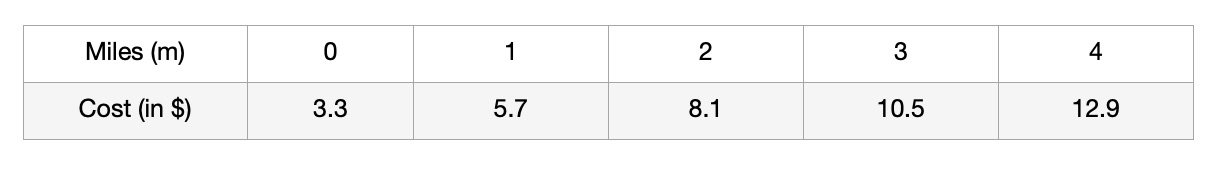
\includegraphics[width=0.9\textwidth,height=\textheight]{images/i.jpeg}

\textbf{Question:} What are the advantages and disadvantages of using a
table instead of a formula or verbal description?

We can also represent the function above using a graph. See below:

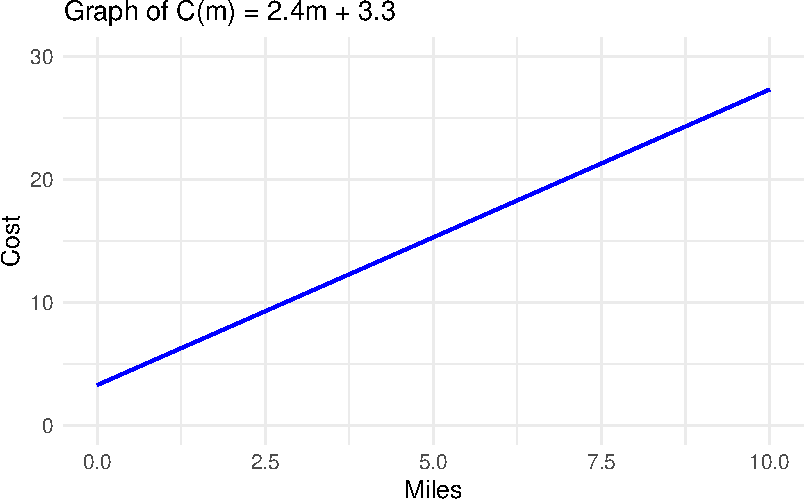
\includegraphics{Intro_LF_files/figure-pdf/unnamed-chunk-1-1.pdf}

Since the cost is dependent on the miles traveled, we call it a
\textbf{\emph{Dependent Variable}}. We call the miles \((m)\) an
\textbf{\emph{Independent Variable}}. By convention, we place the
dependent variable on the horizontal axis (x-axis) and the dependent
variable on the vertical axis (y-axis).

If you ride 0 miles, the cost is \$3.30, giving the coordinate
\((m, C(m))=(0, 3.30)\) on the graph. We call this point, the vertical
or \(C(m)-intercept\) (or \(y-intercept\) in a general graph using \(x\)
and \(y\)).

We call the above function, a \textbf{\emph{Linear Function}} because
its graph produces a straight line. This straight line results because
the change in cost is consistent on any intervals of miles.

In a graph of any linear function, the rate of change is often referred
to as \textbf{\emph{Slope}} because it tells us how steep the line is.
If the rate of change in the taxi scenario given above were, say, 5
dollars per mile, instead of 2.4, the line would be much steeper than it
is. When a linear function is expressed in the form \(f(x)=mx+b\), we
call it \textbf{\emph{slope-intercept form}}. This form is the most
common because it makes it easier to spot the \(slope\) and the
\(y-intercept\) which are important characteristics of linear functions.

\hypertarget{increasing-and-decreasing-functions}{%
\section{Increasing and Decreasing
Functions}\label{increasing-and-decreasing-functions}}

Notice in the above example that as you increase the number of miles,
the cost of the ride goes up. This is because the rate of change (m) is
positive.

Since as you increase the input value, the output value increases, we
say that the function \(C(m)\) is an increasing function. As can be seen
on the graph, the line is rising from left to right. This is because the
rate of change value is positive.

Generally, a linear function is said to be \textbf{\emph{increasing}} if
the slope \(m\) is positive and \textbf{\emph{decreasing}} if the slope
is negative.

\hypertarget{exercises}{%
\section{Exercises}\label{exercises}}

\begin{enumerate}
\def\labelenumi{\arabic{enumi}.}
\tightlist
\item
  Create a real-life scenario that can be modeled by a decreasing linear
  function.
\item
  Write the formula for the function in exercise 1 above.
\item
  Describe how the graph of the function in exercise 2 would look like.
\item
  What would the graph of the function, \(f(x)= 0x+3\) look like?
\item
  Find the formula for the linear function, \(y=f(x)\), graphed below:
\end{enumerate}

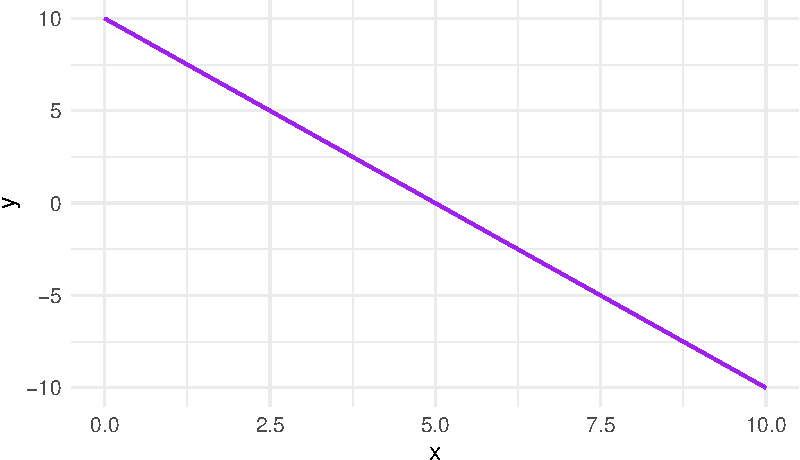
\includegraphics{Intro_LF_files/figure-pdf/unnamed-chunk-2-1.pdf}

\begin{enumerate}
\def\labelenumi{\arabic{enumi}.}
\setcounter{enumi}{5}
\item
  Find the \(y-intercept\) of a linear function whose rate of change is
  2.5 and passes through the point \((3,9)\).
\item
  Marcus currently owns 200 songs in his iTunes collection. Every month,
  he adds 15 new songs. Write a formula for the number of songs, \(N\),
  in his iTunes collection as a function of the number of months, \(m\).
  How many songs will he own in a year if the trend continues?
\end{enumerate}

\hypertarget{rate-of-change}{%
\chapter{Rate of Change}\label{rate-of-change}}

\hypertarget{calculating-rate-of-change}{%
\section{Calculating Rate of Change}\label{calculating-rate-of-change}}

The rate of change (ROC) is perhaps the most important component of any
linear function. As we have seen, it can tell you whether the function
is increasing or decreasing and can be used to create the function
formula (linear model) for a given real life situation. The question
that arises is, ``how can we compute the rate of change from given data
(e.g., from a table?''. In the earlier taxi example, suppose, we did not
know the rate of change but only knew the cost of riding 4 miles and 7
miles. How can we use this information together with the fact that the
function is linear to find the rate of change and even the formula for
the function?

In the next few examples we explore ways of finding the rate of change
and how to use it to create the linear function/model for given
real-life situations. At the end, a formula for computing the rate of
change is provided.

\textbf{Example 1}

The population of a city can be modeled approximately using a linear
function. In 2002, the population was 23,400 and in 2006, it was 27,800.

\begin{enumerate}
\def\labelenumi{\alph{enumi})}
\item
  Find the rate of change of the population for this city.
\item
  What is the formula of the linear function for the scenario? Let \(P\)
  be the population and \(t\) the time in years.
\item
  Assuming the model (function) holds true until 2024, what would be the
  population of the town in 2024?
\end{enumerate}

\textbf{\emph{Solution}}

\begin{enumerate}
\def\labelenumi{\alph{enumi})}
\tightlist
\item
  Since we are told that the population grows linearly, we know that the
  growth between 2002 and 2003 is the same as the growth between 2003
  and 2004, etc. Thus, to find the rate of change (i.e., population
  growth per year), we can divide the population change between 2002 and
  2006 by the number of years as shown:
\end{enumerate}

\[
\begin{aligned} 
Rate\hspace{.04in} of\hspace{.04in} change &=  \frac{pop. \hspace{.04in} in \hspace{.04in} 2006 \hspace{.04in}- pop. \hspace{.04in} in \hspace{.04in} 2002}{2006-2002}\\\\&= 1100\hspace{.04in} people\hspace{.04in} per \hspace{.04in} year
\end{aligned}
\] b) If we use 2002 as the base year(i.e., \(t=0\)), then the FIXED
\(y-intercept\) value in the function is 23,400. We are left with
writing down the function in the form \(f(x)=mx+b\) where \(m\) is the
rate of change and \(b\) is the constant (initial value). Our input
variable is \(t\) so we use it to replace \(x\).

\[f(t) = 1100t+23,400\]

\begin{enumerate}
\def\labelenumi{\alph{enumi})}
\setcounter{enumi}{2}
\tightlist
\item
  For 2024, \(t=22\) years. Thus,
\end{enumerate}

\[
\begin{aligned}
f(22) &= 1100\times22+23,400\\\\&=47,600
\end{aligned}
\]

\textbf{Example 2}

The summit of Africa's largest peak, Mt. Kilimanjaro, has two main ice
fields and a glacier at its peak. Geologists measured the ice cover in
the year 2000 (\(t = 0\)) to be approximately \(1951\hspace{.05in}m^2\);
in the year 2007, the ice cover measured \(1555 \hspace{.05in}m^2\).

\begin{enumerate}
\def\labelenumi{\alph{enumi})}
\item
  Suppose that the amount of ice cover at the peak of Mt. Kilimanjaro is
  changing at a constant average rate from year to year. Find a linear
  model, \(A=f(t)\) whose output is the area, A, in square meters in
  year \(t\) (where \(t\) is the number of years after 2000).
\item
  What do the slope and \(A\)-intercept mean in the model you found in
  (a)? In particular, what are the units on the slope?
\end{enumerate}

\begin{enumerate}
\def\labelenumi{\Alph{enumi})}
\setcounter{enumi}{2}
\tightlist
\item
  Compute \(f(17)\). What does this quantity measure? Write a complete
  sentence to explain.
\end{enumerate}

\begin{enumerate}
\def\labelenumi{\alph{enumi})}
\setcounter{enumi}{3}
\tightlist
\item
  If the model holds further into the future, when do we predict the ice
  cover will vanish?
\end{enumerate}

\textbf{\emph{Solution}}

\begin{enumerate}
\def\labelenumi{\alph{enumi})}
\tightlist
\item
  We begin by finding the rate of change. Since we know that the rate of
  change is constant year after year, we can divide the difference in
  ice coverage between 2007 and 2000 by 7 to get the rate of change per
  year. \begin{align}
  Rate\hspace{.04in} of\hspace{.04in} change &=  \frac{Coverage \hspace{.04in} in \hspace{.04in} 2007 \hspace{.04in}- Coverage \hspace{.04in} in \hspace{.04in} 2000}{2007-2000}\\\\
  &= - 56.57\hspace{.04in} m^2\hspace{.04in} per \hspace{.04in} year
  \end{align} The general format of the function is \(A(t)=mt+b\) where
  \(m\) is the rate of change and \(b\) is the \(A(t)\)-intercept (or
  the value of \(A(0)\) which we know is 1951). Thus, the function is,
\end{enumerate}

\[A(t)=-56.57t + 1951\]

\begin{enumerate}
\def\labelenumi{\alph{enumi})}
\setcounter{enumi}{1}
\item
  The slope means that the ice for every additional year, the ice
  coverage decreases by \(56.57 m^2\). The units are square meters per
  year (\(m^2/year\)). The y intercept means that the initial coverage
  at year zero (when the measurement was first taken) is \(1951 m^2\).
\item
  \(f(17)=(-55.57\times17)+1951=1006.31\); This means that there were
  \(1006.31 mi^2\) of ice coverage on Mt. Kilimanjaro by 2017 (i.e., 17
  years after 2000).
\item
  Remember that \(A(t)\) is the function that gives the ice coverage
  after \(t\) years. Therefore, if the ice cover is zero, it means
  \(A(t)=0\). We compute \(t\) by solving the equation
  \(-56.57t + 1951=0\) for t.
\end{enumerate}

\[
\begin{aligned}
  -56.57t + 1951&=0\\\\
  -56.57t&=-1951\\\\
  t&=\frac{-1951}{-56.57}\\\\
  &=34.49 \hspace{0.04in} years
  \end{aligned}
\]

\hypertarget{a-formula-for-roc}{%
\section{A Formula For ROC}\label{a-formula-for-roc}}

From the foregoing examples, it should be readily clear that, given two
input values \(x_1\) and \(x_2\) such that \(x_1\neq x_2\),

\[
\begin{aligned}
  Rate \hspace{0.04in}of\hspace{0.04in} Change                         
  &=\frac{Change\hspace{0.04in}in\hspace{0.04in}Output}{Change \hspace{0.04in}         
  in\hspace{0.04in}Input}\\ \\
  &=\frac{f(x_2)-f(x_1)}{x_2 - x_1}
  \end{aligned}
\]

\textbf{Example 3}

If \(f(x)\) is a linear function, \(f(3)=−2\), and \(f(8)=1\), find an
equation/formula for the function.

\textbf{\emph{Solution}}

In this problem, we are looking at the input interval between 3 and 8.
Thus, \(x_1=3\) and \(x_2=8\). To find the ROC for \(f(x)\) we proceed
as follows:

\begin{align}
ROC &= \frac{f(x_2)-f(x_1)}{x_2 - x_1}\\\\
&= \frac{f(3)-f(1)}{8 - 3}\\\\
&= \frac{1-(-2)}{5}\\\\
&=\frac{3}{5}
\end{align} Next, the general form of the linear function is
\(f(x)=mx+b\), where \(m\) is the \(ROC\) (aka slope. So, we can write,
\(f(x)=\frac{3}{5}x+b\). To find \(b\), we can use one of the known
values of \(f(x)\), such as \(f(8)\) and solve for \(b\) as follows:

\[
\begin{aligned}
f(8)&=\frac{3}{5}\times (8)+b\\\\
1&=\frac{24}{5}+b\\ \\
b&=1-\frac{24}{5}\\ \\
&=-\frac{19}{5}
\end{aligned}
\]

So, the equation becomes,

\[f(x)=\frac{3}{5}x-\frac{19}{5}\]

\hypertarget{point-slope-equation-format}{%
\section{Point-Slope Equation
Format}\label{point-slope-equation-format}}

The equation \(y=mx+b\) is called the slope-intercept form of a linear
function (equation). In cases where you only know one of the points, say
\((x_1,y_1)\) and the slope \(m\) you can express the equation of the
line as follows:

\[y-y_1=m(x-x_1)\] Where, \((x_1,y_1)\) is the KNOWN point.

After this, you can then rearrange the equation into the slope-intercept
format. You just need to be careful with your algebraic manipulation
when doing this. See example below:

\textbf{Example 4}

A new house was sold for \$296000 8 years after it was purchased. The
original owners calculated that the house appreciated \$2,500 per year
while they owned it. Find a linear function that describes the above
situation if \(x\) is the number of years since the building was
purchased.

\textbf{\emph{Solution}}

Let \(x\) be the number of years and \(C(x)\) be the cost of the house
after \(x\) years.

Note that, we do not know the initial price (i.e., \(b\)) but we know
the \(ROC\) in cost to be 2,500 \$ per year (i.e., a linear function).
We also know the cost after 8 years (i.e, we know one point
\((8, 296,000)\)).

We can use this information and the concept of slope-point format to
write the equation of the line as follows:

\[
\begin{aligned}
y-y_1&=m(x-x_1)\\ \\
y-296,000&=2500(x-8)\\ \\
y-296,000&=2500x-20,000\\ \\
y&=2500x-20000+296,000\\ \\
y&=2500x+276,000
\end{aligned}
\] Note that in the above equation, \(y=C(x)\). So we are done. As a
bonus, we know the cost of the house was \$276,000 eight years ago.

\hypertarget{exercises-1}{%
\section{Exercises}\label{exercises-1}}

\begin{enumerate}
\def\labelenumi{\arabic{enumi}.}
\item
  A town has a population of \(2000\) people at time \(t=0\). In each of
  the following cases, write a formula for the population \(P\),of the
  town as a function of year \(t\).

  \begin{enumerate}
  \def\labelenumii{\alph{enumii}.}
  \tightlist
  \item
    The population increases by 90 people per year.
  \item
    The population increases by 1 percent per year.
  \end{enumerate}
\item
  Find the slope of the line connecting the points \((2,7)\) and
  \((6,11)\). Find the equation of this line.
\item
  Working as an insurance salesperson, Ilya earns a base salary and a
  commission on each new policy, so Ilya's weekly income, \(I\), depends
  on the number of new policies, \(n\), he sells during the week. Last
  week he sold 3 new policies, and earned \$760 for the week. The week
  before, he sold 5 new policies, and earned \$920. Find an equation for
  \(I(n)\), and interpret the meaning of the components of the equation.
\item
  Find a formula for the linear equation graphed below. You can enlarge
  the graph by clicking on it.
\end{enumerate}

\includegraphics{ROC_files/figure-pdf/unnamed-chunk-1-1.pdf}

\begin{enumerate}
\def\labelenumi{\arabic{enumi}.}
\setcounter{enumi}{4}
\item
  An apartment manager keeps careful record of how the rent charged per
  unit corresponds to the number of occupied units in a large complex.
  See the table:
  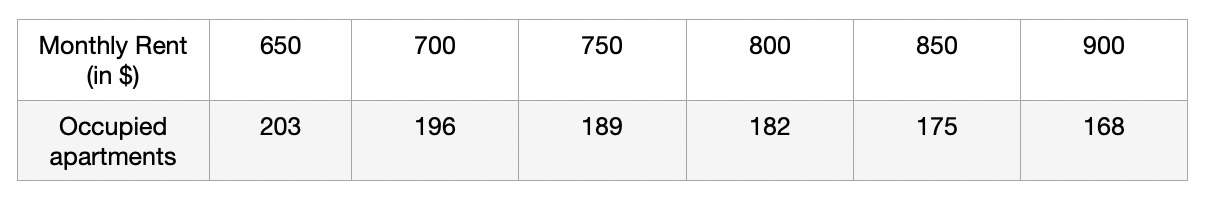
\includegraphics[width=0.5\textwidth,height=\textheight]{images/h.jpeg}

  \begin{enumerate}
  \def\labelenumii{\alph{enumii}.}
  \tightlist
  \item
    Why is it reasonable to say that the number of occupied apartments
    is a linear function of monthly rent?
  \item
    Let \(A\) be the number of occupied apartments and \(R\) the monthly
    rent charged (in dollars). If we let \(A=f(R)\) ,what is the slope
    of the linear function \(f(R)\)? What is the meaning of the slope in
    the context of this question?
  \item
    Determine a formula for \(A=f(R)\).
  \item
    If the rent were to be increased to \$1000, how many occupied
    apartments should the apartment manager expect? How much total
    revenue would the manager collect in a given month when rent is set
    at \$1000?
  \end{enumerate}
\end{enumerate}

\hypertarget{applications}{%
\chapter{Applications}\label{applications}}

\hypertarget{intersecting-lines}{%
\section{Intersecting Lines}\label{intersecting-lines}}

As you saw earlier, graphs are one of the ways commonly used to
represent linear functions. By examining graphs of linear functions, we
learn a lot about the function. For example, we can quickly tell whether
a function is increasing (positive slope), decreasing (negative slope)
or neither (zero slope). We can also get a sense of how fast the output
values are changing with change in the input values. In order to
leverage this benefit of graphs to compare multiple linear functions, it
is often helpful to graph the functions on the same grid.

\textbf{Consider the claim below:}

If two linear functions with \textbf{different} rates of change are
graphed on the same grid, then, the lines must intersect at some point.
Do you think this claim is true? Why or why not?

In the world of business and economics, \textbf{supply} and
\textbf{demand} problems are sometimes modeled using linear functions.
When the demand and supply meet (intersect) we have an equilibrium
point. Consider the following example:

\textbf{Example 1}

The supply, in thousands of items, for custom phone cases can be modeled
by the equation, \(s(p)=0.5+1.2p\) while the demand can be modeled by
\(d(p)=8.7−0.7p\), where p is in the price in dollars. Find the
equilibrium price and quantity, the intersection of the supply and
demand curves.

\textbf{\emph{Solution}}

There are two ways to solve this problem. First, you can set up
\(s(p)=d(p)\) then solve algebraically for \(p\) or simply graph the two
functions then look at the point of intersection.

Let us do both.

\emph{Graphical solution} :

For the graphical solution, you simply graph the two functions (you can
use tools such as desmos or geogebra) and read out the coordinates of
the intersection point.

\includegraphics{LF_Applications_files/figure-pdf/unnamed-chunk-1-1.pdf}

The approximate point of intersection for the graphs is \((4.3,5.6)\).
You can get more accurate values using technology. This intersection is
a pair \((x,y)\) where the first number is the price (input) and the
second if the quantity (output).

\emph{Algebraic solution}:

\begin{align}
  0.5+1.2p&=8.7−0.7p\\ \\
  1.2p+0.7p&=8.7-0.5\\ \\
  1.9p&=8.2\\ \\
  p&=\frac{8.2}{1.9}\\ \\
  &=4.32
\end{align}

Thus, the equilibrium price is approximately \$4.32.

To find the quantity associated with this price, use any of the two
functions to evaluate the output at \(p=4.32\). It does not matter which
function you use because both of them have the same output value at the
point of intersection (a shared point).

\begin{align}
s(4.32)&=0.5+(1.2\times 4.32)\\ \\
&= 5.68
\end{align}

Thus, the two approaches give us the same solution.

\hypertarget{systems-of-equations}{%
\section{Systems of Equations}\label{systems-of-equations}}

\part{Linear Programming}

\hypertarget{geometric-method}{%
\chapter{Geometric Method}\label{geometric-method}}

\hypertarget{introduction-to-linear-programming}{%
\section{Introduction to linear
Programming}\label{introduction-to-linear-programming}}

Managers are often called upon to make complicated decisions. For
example, production managers often make decisions on what products to
manufacture and in what quantities. In making such decisions, the
manager must consider the available resources and how to utilize them
for maximum profit. Note that resources are not limited to raw
materials. They can include labor (human hours), farmland, machinery,
etc. Resources, in general, are always limited and management must
decide how to allocate them in order to get the maximum possible profit.

Linear programming (LP) is one of the most important methods used in
management science to solve problems of the kind describe above. LP
involves maximizing or minimizing a quantity, usually profit or cost,
under some given constraints.

\hypertarget{mixture-problems-charts}{%
\section{Mixture Problems \& Charts}\label{mixture-problems-charts}}

A mixture problem is a problem which includes combining limited
resources to manufacture products that will generate maximum profit for
the company.

These problems are common because most products that we use involve
combining multiple resources in their production. Although there are
other considerations in making production decisions, availability of
resources is one of the most important constraints.

An \textbf{\emph{optimal production policy (OPP)}} is a policy that,

\begin{Shaded}
\begin{Highlighting}[]
\ErrorTok{(}\DataTypeTok{i}\ErrorTok{)} \DataTypeTok{does} \DataTypeTok{not} \DataTypeTok{violate} \DataTypeTok{the} \DataTypeTok{constraints} \DataTypeTok{under} \DataTypeTok{which} \DataTypeTok{the} \DataTypeTok{company} \DataTypeTok{operates} \DataTypeTok{and}\ErrorTok{,}
\ErrorTok{(}\DataTypeTok{ii}\ErrorTok{)} \DataTypeTok{yields} \DataTypeTok{maximum} \DataTypeTok{profit}\KeywordTok{.}
\end{Highlighting}
\end{Shaded}

\textbf{Example 1}

A toy manufacturer can manufacture only skateboards and, only dolls, or
some kind of skateboards and dolls. Skateboards require 5 units of
plastic and can be sold for a profit of \$ 1, while dolls require 2
units of plastic and can be sold for \$0.55 profit. Only 60 units of
plastic are available.

\begin{enumerate}
\def\labelenumi{(\alph{enumi})}
\tightlist
\item
  Make a mixture chart to model this situation.
\item
  What numbers of skateboards and/or dolls should the company make to
  maximize profit?
\end{enumerate}

Before we solve this problem, note that it is a mixture problem because:

\begin{itemize}
\item
  Definite resources are available in limited quantities. The resource
  here is container units of plastic.
\item
  Definite products can be made by combining (mixing) the resources. The
  products here are skateboards and dolls.
\end{itemize}

\textbf{\emph{Solution}}

\begin{enumerate}
\def\labelenumi{\alph{enumi})}
\tightlist
\item
  A mixture is a simple table that shows the resources, products, and
  profit. The chart displays the ``verbal'' information into a format
  that makes it easier to convert the problem to mathematical form
  (equations) that we can then solve. The rows of the mixture chart
  contain the products while the columns contain the resources and the
  profit margin. Below is a mixture chart for the problem above:
\end{enumerate}

\begin{longtable}[]{@{}
  >{\centering\arraybackslash}p{(\columnwidth - 4\tabcolsep) * \real{0.2740}}
  >{\centering\arraybackslash}p{(\columnwidth - 4\tabcolsep) * \real{0.4658}}
  >{\centering\arraybackslash}p{(\columnwidth - 4\tabcolsep) * \real{0.2603}}@{}}
\caption{\textbf{Mixture Chart for dolls and skateboards
problem}}\tabularnewline
\toprule\noalign{}
\begin{minipage}[b]{\linewidth}\centering
Products
\end{minipage} & \begin{minipage}[b]{\linewidth}\centering
Resource(s): Containers of plastic: 60
\end{minipage} & \begin{minipage}[b]{\linewidth}\centering
Profit (per unit)
\end{minipage} \\
\midrule\noalign{}
\endfirsthead
\toprule\noalign{}
\begin{minipage}[b]{\linewidth}\centering
Products
\end{minipage} & \begin{minipage}[b]{\linewidth}\centering
Resource(s): Containers of plastic: 60
\end{minipage} & \begin{minipage}[b]{\linewidth}\centering
Profit (per unit)
\end{minipage} \\
\midrule\noalign{}
\endhead
\bottomrule\noalign{}
\endlastfoot
Skateboard (x units) & 5 & \$ 1.00 \\
Dolls(y units) & 2 & \$ 0.55 \\
\end{longtable}

\begin{enumerate}
\def\labelenumi{\alph{enumi})}
\setcounter{enumi}{1}
\item
  There are several methods of solving linear programming problems such
  as the one provided above. Many of the methods follow the following
  general steps:

  \begin{itemize}
  \tightlist
  \item
    Translating the problem into a mathematical form,
  \item
    Identifying a set of possible solutions (feasible region) and,
  \item
    Identifying a solution that would give us maximum profit, i.e., the
    optimal b production policy.
  \end{itemize}

  We will consider the geometric approach first and discuss its
  advantages as well as limitations then present a more general method
  in the next chapter. After you have understood how these methods work,
  you will have an opportunity to use technology (e.g., Excel
  spreadsheets, and web applications) to solve LP problems. Note,
  however, that technology may not help you in translating the problem
  into mathematical terms. That part is done by humans (YOU).
\end{enumerate}

\hypertarget{the-geometric-method}{%
\section{The Geometric Method}\label{the-geometric-method}}

The geometric method of solving linear programming problems involves
creating a graph to visualize the \textbf{feasible region} (the set of
likely solutions) and then identifying the correct solution from the
feasible region. Since the inequalities involve linear functions, the
feasible region is polygonal in shape. The type of polygon formed
(triangle, quadrilateral, pentagon, etc) depends on the number of
constraints you have.

\begin{Shaded}
\begin{Highlighting}[]
\DataTypeTok{A} \DataTypeTok{feasible} \DataTypeTok{set} \ErrorTok{(}\DataTypeTok{region}\ErrorTok{)} \DataTypeTok{for} \DataTypeTok{an} \DataTypeTok{LP} \DataTypeTok{problem} \DataTypeTok{is} \DataTypeTok{the} \DataTypeTok{collection} \DataTypeTok{of} \DataTypeTok{all} \DataTypeTok{physical}
\DataTypeTok{possible} \DataTypeTok{solution} \DataTypeTok{choices} \DataTypeTok{that} \DataTypeTok{can} \DataTypeTok{be} \DataTypeTok{made}\KeywordTok{.} 
\end{Highlighting}
\end{Shaded}

Let us proceed with the solution to Example 1. We will start by
converting the problem into mathematical terms (inequalities and
equations), creating a feasible region, and then use a technique called
the \textbf{corner point principle} to choose the best solution from the
feasible region.

\hypertarget{convering-mixture-chart-into-mathematical-form}{%
\subsection{Convering Mixture Chart into Mathematical
Form}\label{convering-mixture-chart-into-mathematical-form}}

First, we know that we cannot manufacture negative number of objects
(skateboards of dolls). So, negative numbers are not permitted in this
context. Note however, that 0 is a possible number. Thus, we have two
inequalities;

\[x \ge 0 \hspace{.04in} \text{and} \hspace{.04in} y \ge 0\]

The symbol \(>\) means grater than while \(\ge\) means greater than or
equal to.

We call the above two inequalities \textbf{\emph{minimum constraints}}
because they tell us the minimum that we can have for each product.

Since we have a limited supply of resources (in this case 60 units of
plastic) we must also have inequalities for \textbf{\emph{resource
constraints}}. Since we need 5 units of plastic to manufacture ONE
skateboard, we will need \(5x\) units to manufacture x units of
skateboards. Similarly, we will need \(2y\) units of plastic to
manufacture y dolls. In total, we need \(5x+2y\) units of plastic to
manufacture the dolls and skateboard. This value must not exceed 60.
Thus, we have the inequality,

\[5x+2y\le60\]

Notice that this time, we use the symbol for less than or equal to.

In this problem, we only have 3 inequalities but in a realistic problem,
there would be hundreds or even thousands of them.

The last step in formulating the mathematical model is to make the
\textbf{objective function}. This is the function that connects the
profit to the resources. Since we know that each skateboard results in
\$1.00 profit, we know that x dolls will result in a profit of \(\$1x\)
and y dolls will result in a profit of \(\$0.55x\). We do not know what
the profit is but we know it is a function of both dolls and
skateboards. We can denote the profit as \(P\). So, we have the
equation,

\[P=1x+0.55y\] Notice that the objective function is an
\textbf{equation} (not inequality) that gives a \textbf{specific} amount
of profit as we vary the number of skateboards and dolls. In other
words, \(P\) changes as we change \(x\) and \(y\). So we can determine
the value of \(x\) and\(y\) that would produce maximum \(P\).

\hypertarget{representing-the-feasible-region}{%
\subsection{Representing the Feasible
Region}\label{representing-the-feasible-region}}

After creating the inequalities from the mixture chart, we can draw a
picture to help us visualize the feasible region geometrically. Graphs
are the most commonly used tools for visualizing the feasible region.

Notice that all the three inequalities (i.e., the minimum and resource
constraints) are linear in the sense that when you graph them (assuming
an equal sign) you will get a straight line. To take care of the fact
that the inequalities admit a broad range of values, we,

\begin{enumerate}
\def\labelenumi{\alph{enumi})}
\tightlist
\item
  Use a dotted line if the inequality is strictly less \((<)\) or
  greater \((>)\) and shade the region representing the constraints. For
  example, if \(y>2\), we draw a dotted line for \(y=2\) and shade the
  region \textbf{above} the line on the graph (this is the region that
  obeys the constraint).
\item
  Use a bold line if the inequality allows equality.
\end{enumerate}

Below is a graph of the feasible region for our problem above. We have
shaded the region where x values and y values are greater than 0, as
well as the region where \(5x+2y\) is less than or equal to 60.

\begin{figure}

{\centering 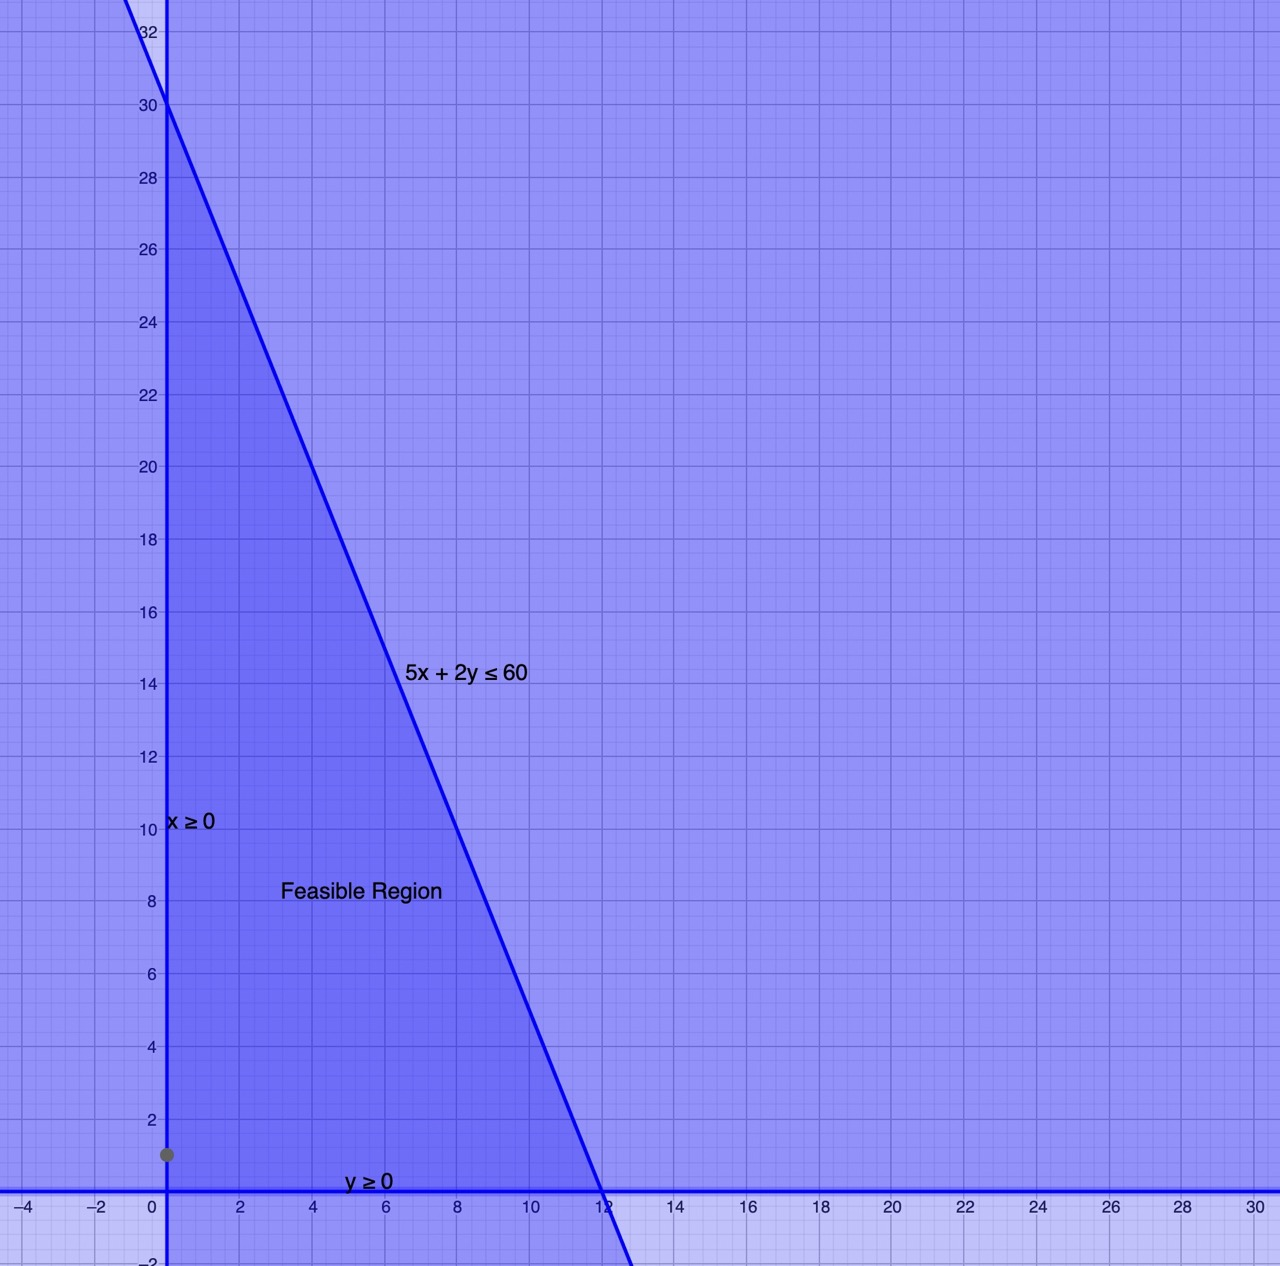
\includegraphics[width=0.8\textwidth,height=\textheight]{images/a.jpeg}

}

\caption{Graph of the Feasible Region}

\end{figure}

All points within the region labelled ``feasible region'' are possible
solutions to our problem in the sense that they do not violate the
constraints. For example, the feasible point \((8,4)\) requires the
company to manufacture 8 skateboards and 4 dolls. This ``solution'' does
not violate any of the constraints given in the problem. To find the
profit associated with this point, we use the objective (profit)
function to compute the profit as follows:

\$\$

\begin{align}
P&=x+0.55y\\
&=8+(0.55\times 4)\\
&=\$10.20
\end{align}

\$\$

Now, it is easy to show that there is a different point within the
feasible region that would yield a higher profit while still obeying the
constraints. Take, for example, the point \((2,20)\) which means 2
skateboards and 20 dolls. The profit for this choice would be higher.
See below:

\$\$

\begin{align}
P&=1.00 x+0.55y\\
&=2+(0.55\times 20)\\
&=\$13.0
\end{align}

\$\$

Choosing a point in the feasible region that would result in maximum
profit (optimal production policy) is not a trivial task. However, there
is an genius technique known as \textbf{\emph{The Corner Point
Principle}} which we discuss next.

\hypertarget{the-corner-point-principle}{%
\subsection{The Corner Point
Principle}\label{the-corner-point-principle}}

The corner point principle has been touted as one of the most important
insights into the theory of linear programming. The principle states
that,

\begin{Shaded}
\begin{Highlighting}[]
\DataTypeTok{In} \DataTypeTok{a} \DataTypeTok{linear} \DataTypeTok{programming} \DataTypeTok{problem}\ErrorTok{,} \DataTypeTok{the} \DataTypeTok{maximum} \DataTypeTok{value} \DataTypeTok{for} \DataTypeTok{the} \DataTypeTok{profit} \DataTypeTok{formula} \DataTypeTok{always}
\DataTypeTok{corresponds} \DataTypeTok{to} \DataTypeTok{a} \DataTypeTok{corner} \DataTypeTok{point} \DataTypeTok{of} \DataTypeTok{the} \DataTypeTok{feasible} \DataTypeTok{region}\KeywordTok{.}
\end{Highlighting}
\end{Shaded}

For our feasible region above, there are \textbf{three corners}. These
corners have coordinates \((0,0)\), \((0,30\), and \((12,0)\). So, we
use the profit function to compute the profit associated with each of
these 3 points and choose the highest as our optimal production policy.
See the calculations below:

For \((0,0)\), the profit would be \(P=1.00 (0)x+0.55(0)=\$0.00\)

For \((0,30)\), the profit would be, \(P=1.00 (0)x+0.55(30)=\$16.50\)

For \((12,0)\), the profit would be, \(P=1.00 (12)x+0.55(0)=\$12.00\)

Therefore, the \textbf{\emph{optimal production policy}} would be to
manufacture 0 skateboards and 30 dolls.

\textbf{NOTE}: In the real world, there would be a lot more corners
which would make this process cumbersome. However, as mentioned earlier,
there are computer programs that can do the job faster and more
efficiently than humans.

\hypertarget{summary-of-the-geometric-method}{%
\subsection{Summary of the Geometric
Method}\label{summary-of-the-geometric-method}}

\begin{enumerate}
\def\labelenumi{\arabic{enumi}.}
\tightlist
\item
  Read the problem carefully to identify resources and products.
\item
  Make a mixture chart for the problem.
\item
  Assign an unknown quantities (often \(x\), and \(y\)) to each product
  and use the mixture chart to write the resource and minimum
  constraints.
\item
  Write the profit formula as well.
\item
  Create a feasible region by graphing ther inequalities (you can use a
  program such as Geogebra or Desmos).
\item
  Find the coordinates of the corner points and evaluate the profit for
  each. The corner that gives maximum profit is the optimal production
  policy.
\end{enumerate}

In the next example, we extend the toy problem above to include one more
resource (person minutes). Read below:

\textbf{Example 2}

A toy manufacturer can manufacture only skateboards and, only dolls, or
some kind of skateboards and dolls. Skateboards require 5 units of
plastic and can be sold for a profit of \$ 1, while dolls require 2
units of plastic and can be sold for \$0.55 profit. Only 60 units of
plastic are available. Furthermore, making one skateboard requires 15
person-minutes while making one doll requires 18-person minutes. There
are only 360person person-minutes available.

\begin{enumerate}
\def\labelenumi{(\alph{enumi})}
\tightlist
\item
  Make a mixture chart to model this situation.
\item
  What numbers of skateboards and/or dolls should the company make to
  maximize profit?
\end{enumerate}

\textbf{\emph{Solution}}

\begin{enumerate}
\def\labelenumi{\alph{enumi})}
\tightlist
\item
  Below is the new mixture chart,
\end{enumerate}

\begin{longtable}[]{@{}
  >{\centering\arraybackslash}p{(\columnwidth - 6\tabcolsep) * \real{0.2603}}
  >{\centering\arraybackslash}p{(\columnwidth - 6\tabcolsep) * \real{0.2466}}
  >{\centering\arraybackslash}p{(\columnwidth - 6\tabcolsep) * \real{0.2466}}
  >{\raggedleft\arraybackslash}p{(\columnwidth - 6\tabcolsep) * \real{0.2466}}@{}}
\toprule\noalign{}
\begin{minipage}[b]{\linewidth}\centering
Products
\end{minipage} & \begin{minipage}[b]{\linewidth}\centering
Resource 1: Plastic: 60
\end{minipage} & \begin{minipage}[b]{\linewidth}\centering
Resource 2: person-minutes 360
\end{minipage} & \begin{minipage}[b]{\linewidth}\raggedleft
Profit
\end{minipage} \\
\midrule\noalign{}
\endhead
\bottomrule\noalign{}
\endlastfoot
Skateboard (x units) & 5 & 15 & \$ 1.00 \\
Dolls(y units) & 2 & 18 & \$ 0.55 \\
\end{longtable}

\begin{enumerate}
\def\labelenumi{\alph{enumi})}
\setcounter{enumi}{1}
\tightlist
\item
  We start by writing down the inequalities (constraints) and the profit
  function. We still have the same minimum constraints as from example
  1: \[x \ge 0 \hspace{.04in} \text{and} \hspace{.04in} y \ge 0\] For
  the resource constraints, we have two inequalities because we have two
  resources: For the plastic, we have \[5x+2y\le60\] For the person
  hours, we have, \[15x + 18y \le 360\] The profit function stays the
  same: \[P=1x+0.55y\] Next, we create a feasible region by graphing the
  inequalities. Notice that this new feasible region is smaller than the
  first and it has four corner points. The fourth point is as a result
  of the new inequality created by the additional resource constraints.
  As indicated earlier, the more resources you have, the more the corner
  points you expect.
\end{enumerate}

\begin{figure}

{\centering 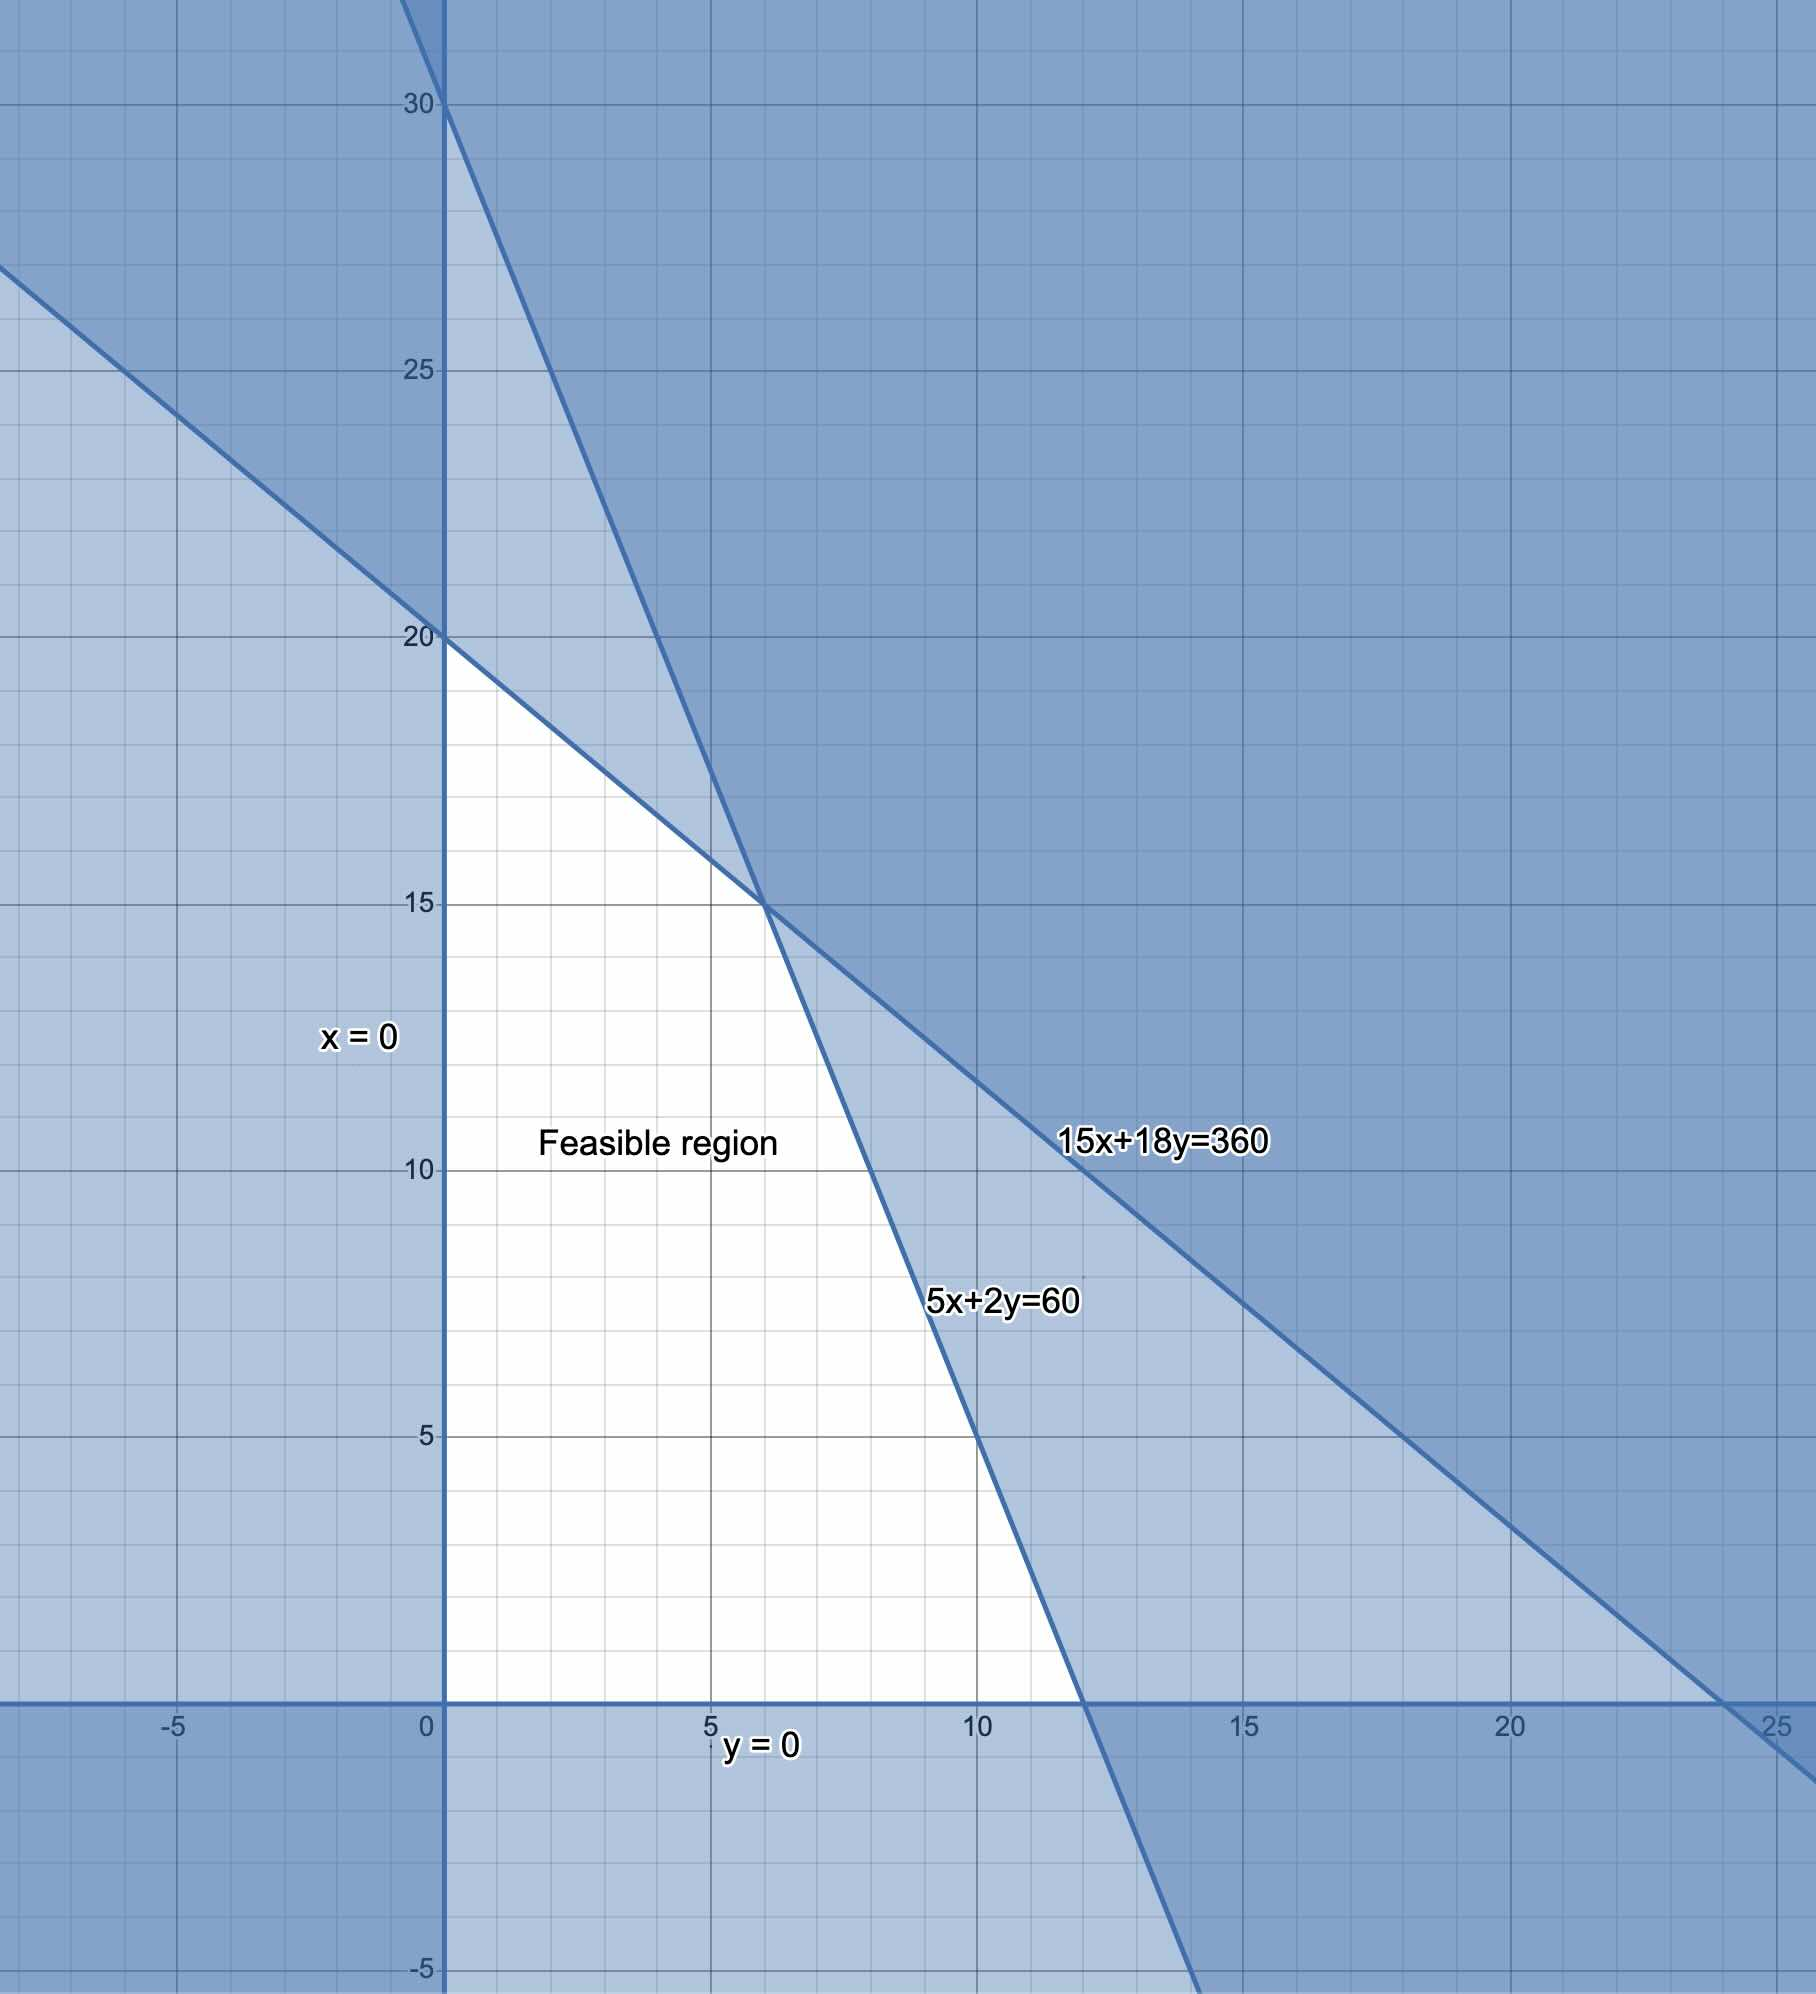
\includegraphics[width=0.9\textwidth,height=\textheight]{images/b.jpeg}

}

\caption{Updated Feasible Region}

\end{figure}

The last step is to use the corner principle to find the optimal
production policy: We check the profits for each of the corner:

For \((0,0)\), the profit would be \(\$0\).

For \((0,20\), the profit would be, \(P=1.00 (0)x+0.55(20)=\$11.00\)

For \((6,15\), the profit would be, \(P=1.00 (6)x+0.55(15)=\$14.50\)

For \((12,0\), the profit would be, \(P=1.00 (12)x+0.55(0)=\$12.00\)

Thus, in this new problem, the optimal production policy is 6
skateboards and 15 dolls for a maximum profit of \$ 14.50.

\hypertarget{exercises-2}{%
\section{Exercises}\label{exercises-2}}

For each description in exercises 1-4, create a mixture table and write
one or more resource constraint inequalities. The unknown to use for
each product is given in parenthesis:

\begin{enumerate}
\def\labelenumi{\arabic{enumi}.}
\tightlist
\item
  Manufacturing one package of hot dogs(x) requires 6 oz of beef, and
  manufacturing one package of bologna (y) requires 4 oz of beef. There
  are 300 oz of beef available.
\item
  It takes 30 ft of 12-in. board to make one bookcase (x); it takes 72
  ft of 12-in. board to make one table(y). There are 420 ft of 12-in.
  board available.
\item
  Manufacturing one salami(x) requires 12 oz of beef and 4 oz of pork.
  Manufacturing one bologna (y) requires 10 oz of beef and 3 oz of pork.
  There are 40 lb of beef and 480 oz of pork available.
\end{enumerate}

For each of the following exercises, graph the feasible region, label
each line segment bounding it with appropriate equation, and give the
coordinates of every corner point.

\begin{enumerate}
\def\labelenumi{\arabic{enumi}.}
\setcounter{enumi}{3}
\item
  \(x\ge 0\) ; \(y\ge 0\); \(2x+y\le10\)
\item
  \(x\ge 0\) ; \(y\ge 0\); \(x+2y\le12\); \(x+2y\le8\)
\item
  \(x\ge 2\) ; \(y\ge 6\); \(3x+2y\le30\)
\item
  Determine whether the points \((2,4)\) and/or \((10,6)\) are points of
  the feasible region in exercises 4, 5, and 6.
\item
  Determine the maximum value of \(P\) given by \(P=3x+2y\) subject to
  the constraints \(x\ge 0\), \(y\ge 0\), \(x\le 7\), and \(y\le 5\).
\item
  A linear programming problem has the following constraints: \(x\ge0\),
  \(y\ge0\), \(5x-y\le15\), and \(4y+x\le24\).

  \begin{enumerate}
  \def\labelenumii{\alph{enumii})}
  \tightlist
  \item
    Without graphing, determine the corner points of the feasible region
    for the LP problem?
  \item
    Sketch a graph of the feasible region.
  \end{enumerate}
\item
  Nuts Galore sells two spiced nut mixtures: Grade A and Grade B. Grade
  A requires 7 oz of peanuts and for every 8 oz of almonds. Grade B
  requires 9 oz of peanuts for every 8 oz of almonds. There are 630 oz
  of peanuts 640 oz of almonds available. Grade A makes Nuts Galore a
  profit of \$1.70, and Grade B makes a profit of \$2.40 per unit
  assembled. How many units of Grade A and Grade B nut mixtures should
  be made to maximize the company's profit, assuming that all the units
  can be sold?
\item
  Find the maximum value of \(P\) where \(P=3x+2y\) subject to the
  constraints \(x\ge3\), \(y\ge2\), \(x+y\le10\), and \(2x+3y\le24\).
\item
  A clothing manufacturer has 600 yd of cloth available to make shirts
  and decorated vests. Each shirt requires 3 yd of material and provides
  a profit of \$5. Each vest requires 2 yd of material and provides a
  profit of \$2. The manufacturer wants to guarantee that under all
  circumstances, there are minimums of 100 shirts and 30 vests produced.
  How many of each garment should be made to maximize the profit? If
  there are no minimum quantities, how, if at all, does the optimal
  production policy change?
\item
  A paper recycling company uses scrap cloth and scrap paper to make two
  different grades of recycled paper. A single batch of grade A recycled
  paper is made from 25 lb of scrap cloth and 10 lb of scrap paper,
  whereas one batch of grade B recycled paper is made from 10 lb of
  scrap cloth and 20 lb of scrap paper. The company has 100 lb of scrap
  cloth and 120 lb of scrap paper on hand. A batch of grade A paper
  brings a profit of \$500, whereas a batch of grade B paper brings a
  profit of \$250. What amounts of each grade should be made? How, if at
  all, do the maximum profit and optimal production policy change if the
  company is required to produce at least one batch of each type?
\item
  Courtesy Calls makes telephone calls for businesses and charities. A
  profit of \$0.50 is made for each business calls and \$0.40 for each
  charity call.It takes 4 min (on average) to make a business call and 6
  min (on average) to make a charity call. If there are 240 min of
  calling time to be distributed each day, how should that time be spent
  so that Courtesy Calls makes a maximum profit? What changes, if any,
  occur in the maximum profit and optimal production policy if they must
  make at least 12 business calls and 10 charity call every day?
\item
  A factory manufactures chairs and tables, each requiring the use of
  three operations: Cutting, Assembly, and Finishing. The first
  operation can be used at most 39 hours; the second at most 42 hours;
  and the third at most 23 hours. A chair requires 1 hour of cutting, 2
  hours of assembly, and 1 hour of finishing; a table needs 2 hours of
  cutting, 1 hour of assembly, and 1 hour of finishing. If the profit is
  \$20 per unit for a chair and \$30 for a table, how many units of each
  should be manufactured to maximize profit?
\end{enumerate}

\hypertarget{the-simplex-method}{%
\chapter{The Simplex Method}\label{the-simplex-method}}

\hypertarget{introduction-to-simplex-method}{%
\section{Introduction to Simplex
Method}\label{introduction-to-simplex-method}}

As stated earlier, Linear Programming is one of the most commonly used
methods for solving practical problems in business and even in
government. However, the problems we have considered so far had a
maximum of two products and relatively small feasible regions and few
corner points. Many real life problems often involve much more products
and result in very big feasible regions with hundreds or even thousands
of corner points.

The simplex method provides a more general method of solving LP programs
without relying on a \textbf{physical} feasible region. Consider the
following LP problem through which we will discuss the details of the
simplex method:

\textbf{Example 1}

A factory manufactures chairs, tables and bookcases each requiring the
use of three operations: Cutting, Assembly, and Finishing. The first
operation can be used at most 600 hours; the second at most 500 hours;
and the third at most 300 hours. A chair requires 1 hour of cutting, 1
hour of assembly, and 1 hour of finishing; a table needs 1 hour of
cutting, 2 hours of assembly, and 1 hour of finishing; and a bookcase
requires 3 hours of cutting, 1 hour of assembly, and 1 hour of
finishing. If the profit is \$20 per unit for a chair, \$30 for a table,
and \$25 for a bookcase, how many units of each should be manufactured
to maximize profit?

Let us start by creating a mixture chart for the problem:

\begin{longtable}[]{@{}
  >{\raggedright\arraybackslash}p{(\columnwidth - 8\tabcolsep) * \real{0.1494}}
  >{\centering\arraybackslash}p{(\columnwidth - 8\tabcolsep) * \real{0.2069}}
  >{\centering\arraybackslash}p{(\columnwidth - 8\tabcolsep) * \real{0.2184}}
  >{\centering\arraybackslash}p{(\columnwidth - 8\tabcolsep) * \real{0.2299}}
  >{\centering\arraybackslash}p{(\columnwidth - 8\tabcolsep) * \real{0.1609}}@{}}
\toprule\noalign{}
\begin{minipage}[b]{\linewidth}\raggedright
Products
\end{minipage} & \begin{minipage}[b]{\linewidth}\centering
Resource:

Cutting(600hrs)
\end{minipage} & \begin{minipage}[b]{\linewidth}\centering
Resource:

Assembly(500hrs)
\end{minipage} & \begin{minipage}[b]{\linewidth}\centering
Resource:

Finishing(300hrs)
\end{minipage} & \begin{minipage}[b]{\linewidth}\centering
Profit (\$)
\end{minipage} \\
\midrule\noalign{}
\endhead
\bottomrule\noalign{}
\endlastfoot
Chairs & 1 & 1 & 1 & 20 \\
Tables & 1 & 2 & 1 & 30 \\
Bookcases & 3 & 1 & 1 & 25 \\
\end{longtable}

Next, we make the constraint inequalities assuming that the company
makes \(x\) chairs, \(y\) tables, and \(z\) bookcases. Note that using
\(x,y\), and \(z\) is not advisable when you have more than 3 variables.
It is recommended you use \(x_1, x_2, x_3,...\)

\textbf{Minimum constraints:} Chairs: \(x\ge 0\) Tables: \(y\ge 0\)
Bookcases: \(z\ge 0\).

\textbf{Resource constraints:} For cutting: \(x+y+3z\le600\) For
assembly: \(x+2y+z\le500\) For finishing: \(x+y+z\le300\)

\textbf{Things to Note}

\begin{itemize}
\tightlist
\item
  Unlike the problems encountered in the previous chapter, this problem
  includes 3 variables \((x,y, z).\) This means that, we would have to
  create a three dimensional graph to visualize the feasible region- a
  task that is impossible for humans to execute by hand.
\item
  Most application problems include way more than 3 variables, which
  means we would need a multidimensional graph to visualize the feasible
  region.
\item
  The simplex method provides an algorithmic method that solves this
  type of problems without needing to create a visual feasible region.
  The method can also be used to solve problems in the previous chapter.
\item
  The technical details of the simplex method are beyond the scope of
  the course but the algorithm itself is relatively easy to execute once
  you learn it.
\end{itemize}

You should try this problem on your own (see exercises) once you have
understood the simplex method. For now, the step-by-step procedure of
the simplex algorithm is presented.

\hypertarget{step-by-step-simplex-method}{%
\section{Step-by-Step Simplex
Method}\label{step-by-step-simplex-method}}

We want to walk through the simplex method step-by-step until we find an
optimal production policy and the maximum profit.

Consider the example below:

\textbf{Example 2}

Maximize the function \(P=3x+4y+z\) subject to the conditions

\[3x+10y+5z \le 120 \] \[5x+2y+8z \le 6\] \[8x+10y+3z \le 105\]

\textbf{\emph{Problem Posing:}} Note that this problem does not have a
real world context, before you proceed, please write a real life LP
problem that might suit the given profit function and constraints.

\textbf{Step 1:} Convert the inequalities to equations by adding
\textbf{slack variables} and rewrite the profit function so that the
constant value is on the right hand side of the equation:
\[3x+10y+5z+s_1 = 120 \] \[5x+2y+8z +s_2= 6\] \[8x+10y+3z +s_3= 105\]
\[-3x-4y-z+P\] Slacks allow us to convert inequalities to equations by
filling up the amount by which a quantity falls short of another. For
example, \(s_1\) is the amount by which the quantity \(3x+10y+5z\) falls
short of 120. So, by adding \(s_1\) to \(3x+10y+5z\) we achieve the
equality. sh

\textbf{Step 2:} Create the initial \textbf{simplex tableau}. In the
tableu, each equation appears in its own row with the profit function
appearing as the last row. See table below:

\begin{figure}

{\centering 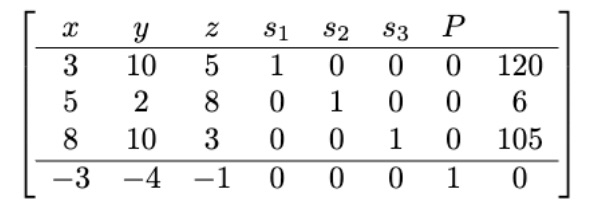
\includegraphics[width=0.5\textwidth,height=\textheight]{images/c.jpeg}

}

\caption{Initial Tableau}

\end{figure}

\textbf{Step 3:} Choose the pivot column. The most negative entry in the
last row is -4 which is in column 2. So, column 2 is our pivot column.
See below:

\begin{figure}

{\centering 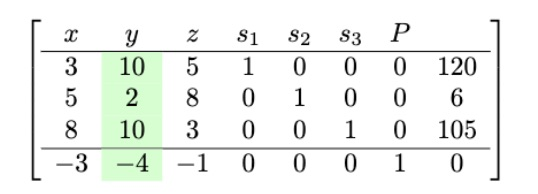
\includegraphics[width=0.5\textwidth,height=\textheight]{images/d.jpeg}

}

\caption{Tableau showing Pivot column}

\end{figure}

Why do we choose the most negative element in the last row?

The most negative entry in the bottom row represents the largest
coefficient in the objective function - the coefficient whose entry will
increase the value of the objective function the quickest. Remember this
is a maximization problem.

\textbf{Step 4:} Find the pivot row. To find the pivot row, divide the
values on the far right by values of the pivot column. The row with the
smallest quotient will be your pivot row. In this case, \[120/10=12\]
\[6/2=3\] \[105/110=10.5\] The smallest quotient here is 3, which means
the pivot row is row 2. The matrix below highlight the picot row:

\begin{figure}

{\centering 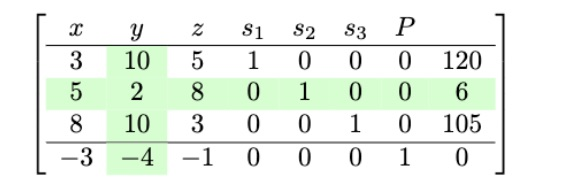
\includegraphics[width=0.5\textwidth,height=\textheight]{images/e.jpeg}

}

\caption{Pivot row and column}

\end{figure}

Why does the smallest quotient identify a row? Using the quotients to
identify the pivot element guarantees that we do not violate the
constraints as we proceed with the algorithm.

\textbf{Step 5:} The 2 at the intersection of row 2 and column 2 is
called a pivot element. We want to perform row operations to make it a
1. To do this, we simply divide the whole of row 2 by 2. This can be
represented as \(\frac{1}{2}R_2 \mapsto R_2\). This means that the new
row 2 will be half of the previous row 2.

\(\frac{1}{2}\times(5,2,8,0,1,0,0,6)=(2.5,1,4,0,.5,0,0,3)\)

The new tableau becomes,

\begin{figure}

{\centering 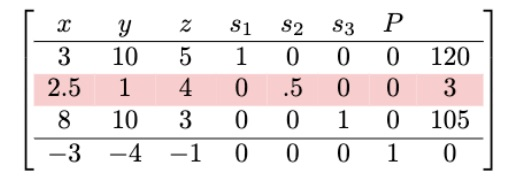
\includegraphics[width=0.5\textwidth,height=\textheight]{images/f.jpeg}

}

\caption{Unitize pivot element}

\end{figure}

\textbf{Step 6:} We perform row operations to convert every entry above
and below the new pivot element (1) into a 0. The following operations
will achieve this:

\begin{itemize}
\tightlist
\item
  The new row 1 will be the difference between row and and 10 times row
  2 i.e., \(R_1 - 10R_2\mapsto R_1\).
\item
  The new row 3 will be the difference between the current row 3 and 10
  times row 2.e., \(R_3 - 10R_2\mapsto R_3\).
\item
  The new row 4 will be the current row 4 plus 4 times row 2 i.e.,
  \(R_4 + 4R_2\mapsto R_4\).
\end{itemize}

We perform the actual computations below:

\(R_1 - 10R_2\mapsto R_1\):
\((3,10,5,1,0,0,0,120) - 10(2.5,1,4,0,0.5,0,0,3)=(-22,0,-35,1,-5,0,0,90)\).

\(R_3 - 10R_2\mapsto R_3\):
\((8,10,3,0,0,1,0,105) - 10(2.5,1,4,0,0.5,0,0,3)=(17,0,-37,0,-5,1,0,75)\).

\(R_4 + 4R_2\mapsto R_4\):
\((-3,-4,-1,0,0,0,1,0) + 4(2.5,1,4,0,0.5,0,0,3)=(7,0,15,0,2,0,1,12)\).

Now we put these new rows into our tableau. See below:

\begin{figure}

{\centering 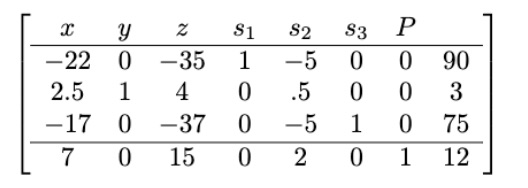
\includegraphics[width=0.5\textwidth,height=\textheight]{images/g.jpeg}

}

\caption{One more Tableau}

\end{figure}

\textbf{Notice that} the last row has no negative numbers. This means we
are done and we can directly read our solution. If there were any
negative numbers left on the last row, you would have to do the process
one more time (i.e., find new pivot column and row then perform
subsequent row operations). This process continues until there are no
negative numbers on the last row.

\textbf{Step 7:} Read the solution from the final tableau. Every column
with a ``1's'' and ``0's'' would give us a value for a variable. In our
case above,

\(y=3, s_1=90, s_3=75, P=12\)

All the others (i.e., \((x,z,s_2)\)) will be zero.

This solution basically means, make 3 units of product \(y\), and zero
product \(x\) and \(z\).

\hypertarget{summary-of-the-simplex-method}{%
\subsection{Summary of the Simplex
Method}\label{summary-of-the-simplex-method}}

Below is a summary of the simplex method for maximization problems in
LP:

\begin{enumerate}
\def\labelenumi{\alph{enumi})}
\tightlist
\item
  Set up the problem. That is, convert the problem into mathematical
  terms. This involves creating the constraint inequalities and the
  objective function.
\item
  Convert the inequalities into equations. This is done by adding one
  slack variable for each inequality.
\item
  Construct the initial simplex tableau with the objective function as
  the bottom row. d)Identify the pivot column. The most negative entry
  in the bottom row identifies the pivot column.
\item
  Calculate the quotients. The smallest quotient identifies a row. The
  element in the intersection of the column identified in step 4 and the
  row identified in this step is identified as the pivot element. The
  quotients are computed by dividing the far right column by the
  identified column in step 4. A quotient that is a zero, or a negative
  number, or that has a zero in the denominator, is ignored.
\item
  Perform pivoting to make all other entries in this column zero.
\item
  When there are no more negative entries in the bottom row, we are
  finished; otherwise, we start again from step (d).
\item
  Read off your answers. Get the variables using the columns with 1 and
  0s. All other variables are zero. The maximum value you are looking
  for appears in the bottom right hand corner.
\end{enumerate}

\hypertarget{a-short-trip-back}{%
\section{A Short Trip Back}\label{a-short-trip-back}}

Let us use the simplex method to solve \textbf{example 2} from the
previous chapter. For your convenience the example is repeated below:

\textbf{Example 3}

A toy manufacturer can manufacture only skateboards and, only dolls, or
some kind of skateboards and dolls. Skateboards require 5 units of
plastic and can be sold for a profit of \$1.00, while dolls require 2
units of plastic and can be sold for \$0.55 profit. Only 60 units of
plastic are available. Furthermore, making one skateboard requires 15
person-minutes while making one doll requires 18-person minutes. There
are only 360person person-minutes available.

\textbf{\emph{Solution}}

Recall that we had generated the following resource inequalities:

\(5x+2y\le 60\)

\(15x+18y\le360\) (Simplifies to \(5x+6y\le120\) by dividing through by
3)

We also had the following profit function: \(P=1.00x+0.55y\)

Our first step is to convert the inequalities to equations by adding
slack variables and rewriting the profit function:

\(5x+2y+s_1= 60\)

\(5x+6y+s_2=120\)

\(-1x-0.55y+P=0\)

Thus, our initial tableau on which we shall perform row operations is:

\begin{bmatrix}
x & y & s_1&s_2&P & | \\
\hline
5 & 2 & 1 & 0 & 0 & |& 60 \\
5 & 6 & 0 & 1 & 0 & | & 120\\
\hline
-1 & -0.55 & 0 & 0 & 1 & |& 0
\end{bmatrix}

Next, we find the pivot element by identifying the pivot column and row.

The most negative entry in the last row is \(-1\) and so the first
column is our pivot column:

\begin{bmatrix}
x & y & s_1&s_2&P & | \\
\hline
\color{red}5 & 2 & 1 & 0 & 0 & |& 60 \\
\color{red}5 & 6 & 0 & 1 & 0 & | & 120\\
\hline
\color{red}-1 & -0.55 & 0 & 0 & 1 & |& 0
\end{bmatrix}

To find the pivot row, we compute following quotients :
\(\frac{60}{5}=12\); \(\frac{360}{5}=72\). Thus, our pivot row is row 1.

\begin{bmatrix}
x & y & s_1&s_2&P & | \\
\hline
\color{red}\textbf5 & \color{red}2 & \color{red}1 & \color{red}0 & \color{red}0 & |& \color{red}60 \\
\color{red}{5} & 6 & 0 & 1 & 0 & | & 120\\
\hline
\color{red}-1 & -0.55 & 0 & 0 & 1 & |& 0
\end{bmatrix}

Our pivot element is, therefore, the \(5\) in the first row. Next
perform row operations to make the element a \(1\). The operation to
achieve this goal is \(\frac{1}{5}R_2\) (i.e., we multiply the entire
row 2 by one fifth). The new tableau becomes,

\begin{bmatrix}
x & y & s_1&s_2&P & | \\
\hline
\color{red}\textbf{1} & 0.4 & 0.2 & 0 & 0 & |& 12\\
5 & 6 & 0 & 1 & 0 & | & 120\\
\hline
-1 & -0.55 & 0 & 0 & 1 & |& 0
\end{bmatrix}

Next, we perform row operations that will convert all entries of column
1 (except our pivot element) to 0. Let us start by targeting the 5. The
operation \(R_2-5R_1 \mapsto R_2\) (\textbf{replace row 1 by row 2 minus
five times row 1}) will achieve our desired goals. See the new tableau
below:

\begin{bmatrix}
x & y & s_1&s_2&P & | \\
\hline
\color{red}\textbf{1} & 0.4 & 0.2 & 0 & 0 & |& 12\\
\color{red}\textbf{0} & 4 & -5 & 1 & 0 & | & 60\\
\hline
-1 & -0.55 & 0 & 0 & 1 & |& 0
\end{bmatrix}

Next, we perform the operation \(R_3+R_1 \mapsto R_3\), which achieve
the goal of converting the \(-1\) on the last row into a zero. Here is
the new tableau:

\begin{bmatrix}
x & y & s_1&s_2&P & | \\
\hline
\color{red}\textbf{1} & 0.4 & 0.2 & 0 & 0 & |& 12\\
\color{red}\textbf{0} & 4 & -5 & 1 & 0 & | & 60\\
\hline
\color{red}\textbf{0} & -0.15 & 0.2 & 0 & 1 & |& 12
\end{bmatrix}

Since the last row still have a negative entry (i.e., \(-1\)), we repeat
the process one more time:

Our new pivot column is column 2 and the pivot row is row 2 (you should
verify this). Thus, our pivot element is the 4 in row 2.

To convert the 4 into a 1, we perform the operation \(\frac{1}{4}R_2\)
(i.e., multiply the entire row by one fourth). Here is the new tableau:

\begin{bmatrix}
x & y & s_1&s_2&P & | \\
\hline
1 & 0.4 & 0.2 & 0 & 0 & |& 12\\
0 & \color{red}\textbf{1} & -1.25 & 0.25 & 0 & | & 15\\
\hline
0 & -0.15 & 0.2 & 0 & 1 & |& 12
\end{bmatrix}

Next, we convert the - 0.15 into 0 by performing the operation
\(R_3+0.15R_2\mapsto R_3\). The new tableau becomes,

\begin{bmatrix}
x & y & s_1&s_2&P & | \\
\hline
1 & 0.4 & 0.2 & 0 & 0 & |& 12\\
0 & \color{red}\textbf{1} & -1.25 & 0.25 & 0 & | & 15\\
\hline
0 & \color{red}\textbf{0} & 0.0125 & 0.0375 & 1 & |& 14.25
\end{bmatrix}

Finally, we convert the 0.4 into a 0 by performing the operation
\(R_1-0.4R_2\mapsto R_1\). The new tableau becomes:

\begin{bmatrix}
x & y & s_1&s_2&P & | \\
\hline
1 & \color{red}\textbf{0} & 0.7 & 0.1 & 0 & |& 6\\
0 & \color{red}\textbf{1} & -1.25 & 0.25 & 0 & | & 15\\
\hline
0 & \color{red}\textbf{0} & 0.0125 & 0.0375 & 1 & |& 14.25
\end{bmatrix}

Notice now that there is no negative entry on the last row. You can now
read off the solutions from the columns with 1's and 0's.

\begin{align}
x&=6\\
y&=15
\end{align}

Which means that the \textbf{optimal production policy} will be
manufacturing 6 skateboards and 15 dolls. The maximum profit will be:
\(P=1.00(6)+0.55(15)=\$14.25\).

The profit can also be read off directly from the tableau above since
the P column has only 0's and 1's.

The above solution is exactly the as the one obtained using the
geometric method in the previous chapter.

\hypertarget{exercises-3}{%
\section{Exercises}\label{exercises-3}}

\begin{enumerate}
\def\labelenumi{\arabic{enumi})}
\tightlist
\item
  Consider the following tableau and answer the questions thereafter.
  Perform row operations to achieve the the results in (a) to (c):
\end{enumerate}

\begin{bmatrix}
x_1 & x_2 & x_3 & s_1 & s_2 & s_3 &P & |&2\\
\hline
1 & 0 & 7 & 1 & 0 & 0 &0& |&5 \\
0 & 1 & 5 & 0 & 1 & 0&0& |&8\\
3 & 1 & 6 & 0 & 0 & 1&0& |&19\\
\hline
-2 & 1 & -1 & 0 & 0 & 0&1& |&0
\end{bmatrix}

\begin{enumerate}
\def\labelenumi{\alph{enumi})}
\tightlist
\item
  Convert the 3 in row 3 into a 1.
\item
  Using the tableau in (a) convert the 1 in row 1 into a 0.
\item
  Convert the -2 in row 4 of the tableau in (b) into a zero.
\end{enumerate}

\begin{enumerate}
\def\labelenumi{\arabic{enumi})}
\setcounter{enumi}{1}
\item
  Find the pivot column, row, and element for the each of the following
  tableaux:

  \begin{enumerate}
  \def\labelenumii{\alph{enumii})}
  \tightlist
  \item
  \end{enumerate}

  \begin{bmatrix}
  x_1 & x_2 & x_3 & s_1 & s_2 & s_3& P& |&\\
  \hline
  7 & 1 & 4 & 1 & 0 & 0& 0 & |&9\\
  0 & 1 & 5 & 0 & 1 & 0& 0& |&3\\
  3 & 1 & 6 & 0 & 0 & 1& 0& |&2\\
  1 & 0 & 7 & 0 & 0 & 0 & 0& |&1\\
  \hline
  4 & -3 & -7 & 0 & 0 & 0& 1& |&0
  \end{bmatrix}

  \begin{enumerate}
  \def\labelenumii{\alph{enumii})}
  \setcounter{enumii}{1}
  \tightlist
  \item
  \end{enumerate}

  \begin{bmatrix}
  x_1 & x_2 & x_3 & s_1 & s_2 & s_3& P& |&\\
  \hline
  4 & 1 & 3 & 1 & 0 & 0& 0 & |&9\\
  0 & 6 & 17 & 0 & 1 & 0& 0& |&3\\
  1 & 2 & 1 & 0 & 0 & 1& 0& |&2\\
  7 & 9 & 3 & 0 & 0 & 0 & 1& |&1\\
  \hline
  1 & -3 & -2 & 0 & 0 & 0& 1& |&0
  \end{bmatrix}
\item
  Create an initial tableau from each of the following set of constraint
  inequalities and the given profit function:

  \begin{enumerate}
  \def\labelenumii{\alph{enumii})}
  \item
    \(P=x+y\) \(-x+y\le4\) \(2x+y\le20\) \(2x-y\le2\)
  \item
    \(P = 4x_1 + x_3 + x_3\) \(x_1 + 2x_2 + 3x_3 \le 6\)
    \(2x_1 + x_2 + x_3 \le3\) \(x_1 + x_2 + x_3 \le2\)
  \item
    \(P = 2x_1 + 2x_3 + 5x_3\) \(x_1 + x_3 \le 2\) \(x_2 + x_3 \le 4\)
    \(x_1 + 2x_3 \le 3\)
  \end{enumerate}
\end{enumerate}

\begin{enumerate}
\def\labelenumi{\arabic{enumi})}
\setcounter{enumi}{3}
\item
  For the following tableaus, write the constraint inequalities and the
  profit function.

  \begin{enumerate}
  \def\labelenumii{\alph{enumii})}
  \tightlist
  \item
  \end{enumerate}

  \begin{bmatrix}
  x_1 & x_2 & x_3 & s_1 & s_2 & s_3 &P &|& \\
  \hline
  3 & 1 & 5 & 1 & 0 & 0&0 &|& 12 \\
  4 & 0 & 2 & 0 & 1 & 0&0 &|& 7\\
  6 & 1 & 0 & 0 & 0 & 1&0 &|& 13\\
  \hline
  -9 & -3 & 1 & 0 & 0 & 0&1 &|& 0
  \end{bmatrix}

  \begin{enumerate}
  \def\labelenumii{\alph{enumii})}
  \setcounter{enumii}{1}
  \tightlist
  \item
  \end{enumerate}

  \begin{bmatrix}
  x_1 & x_2 & x_3 & s_1 & s_2 & s_3 &P &|& \\
  \hline
  2 & 1 & 0 & 1 & 0 & 0&0 &|& 12 \\
  5 & 1 & 5 & 0 & 1 & 0&0 &|& 7\\
  6 & 2 & 1 & 0 & 0 & 1&0 &|& 13\\
  \hline
  3 & -2 & 1 & 0 & 0 & 0&1 &|& 0
  \end{bmatrix}
\end{enumerate}

\begin{enumerate}
\def\labelenumi{\arabic{enumi}.}
\setcounter{enumi}{4}
\tightlist
\item
  Create the inequalities, profit function, and the initial tableau for
  the following scenario: A farmer has 100 acres of land on which she
  plans to grow wheat and corn. Each acre of wheat requires 4 hours of
  labor and \$20 of capital, and each acre of corn requires 16 hours of
  labor and \$40 of capital. The farmer has at most 800 hours of labor
  and \$2400 of capital available. The profit from an acre of wheat is
  \$80 and from an acre of corn is \$100. The farmer needs to maximize
  her profit.
\end{enumerate}

\begin{enumerate}
\def\labelenumi{\arabic{enumi})}
\setcounter{enumi}{5}
\item
  Solve the following LP problems using the simplex method:

  \begin{enumerate}
  \def\labelenumii{\alph{enumii})}
  \tightlist
  \item
    Maximize \(P=x+y\) subject to:
  \end{enumerate}

  \begin{align}
  -x+y &\le4 \\
  2x+y &\le20\\
  2x-y &\le2
  \end{align}

  \begin{enumerate}
  \def\labelenumii{\alph{enumii})}
  \setcounter{enumii}{1}
  \tightlist
  \item
    Maximize \(P = 4x_1 + x_3 + x_3\) subject to:
  \end{enumerate}

  \begin{align}
   x_1 + 2x_2 + 3x_3 \le 6\\
   2x_1 + x_2 + x_3 \le3 \\
   x_1 + x_2 + x_3 \le2
  \end{align}
\end{enumerate}

\begin{enumerate}
\def\labelenumi{\arabic{enumi}.}
\setcounter{enumi}{6}
\item
  A factory manufactures chairs, tables and bookcases each requiring the
  use of three operations: Cutting, Assembly, and Finishing. The first
  operation can be used at most 600 hours; the second at most 500 hours;
  and the third at most 300 hours. A chair requires 1 hour of cutting, 1
  hour of assembly, and 1 hour of finishing; a table needs 1 hour of
  cutting, 2 hours of assembly, and 1 hour of finishing; and a bookcase
  requires 3 hours of cutting, 1 hour of assembly, and 1 hour of
  finishing. If the profit is \$20 per unit for a chair, \$30 for a
  table, and \$25 for a bookcase, how many units of each should be
  manufactured to maximize profit?
\item
  How many acres of each crop should the farmer in problem 5 above plant
  to maximize her profit? Use the simplex method and show all the steps.
\end{enumerate}

\hypertarget{the-transportation-problem}{%
\chapter{The Transportation Problem}\label{the-transportation-problem}}

\hypertarget{introduction-1}{%
\section{Introduction}\label{introduction-1}}

Consider the following scenarios:

\textbf{Scenario 1:} After a long weekend holiday in your city, a
scooter company has extra scooters in some part of the city and too few
in others. The company is faced with the problem of reshuffling the
scooters at a minimal cost so that each part of the city has the right
number for their clients.

\textbf{Scenario 2:} A college has many campuses in a given state and
materials (such as books) are often shared among the campuses. Because
the calendars for each campus differs slightly, there are more resources
in some campuses than others at some given point. The college needs to
transport the resources between campuses to ensure student needs at each
campus are met while keeping the transportation cost as low as possible.

\textbf{Scenario 3:} A huge car manufacturer has three manufacturing
plants and several sales outlets at various locations in the country.
Each outlet needs a specific number of cars. The cost of transporting
the cars from different plants to different sales outlets is known. How
should the company transport the cars while inuring minimum cost?

\textbf{\emph{Definitions}}

Problems of the kind given in the three scenarios above are called
\textbf{Transportation problems}. Companies often face such kind of
problems on a day to day basis. Transportation problems (TPs) are a
special type of linear programming problems where the goal is to
minimize cost of transporting goods/services from a number of
sources/origins (such as manufacturing plants) to a number of
destinations/outlets (such as stores).

\begin{itemize}
\item
  \textbf{Supply:} This refers to the maximum number of products that
  can be shipped from the sources. Different sources may supply
  different amounts of a product.
\item
  \textbf{Demand:} this refers to the minimum number of products that
  the destinations/outlets require. Again, different outlet often have
  different demands.
\item
  \textbf{Rim conditions:} We use the term \textbf{rim conditions} to
  refer to this situation where a specific number can be supplied from
  different sources and a specific number is required at different
  destinations. The rim conditions are satisfied when all units that can
  be supplied have been supplied and all demand requirements for each
  outlet have been met.
\item
  \textbf{TP Tableau:} A transportation problem tableau is a table
  showing the sources, supply quantities for each source, destinations,
  demands for each destination, and the costs for shipping between each
  source and destination. The more units you ship the higher the cost.
\item
  \textbf{Feasible solution:} A solution for a transportation problem
  that does not violate the rim conditions. In other words, all units
  are supplied out and all stores' demands are met.
\item
  \textbf{Optimal Solution:} A feasible solution that guarantees the
  minimum cost of transportation.
\end{itemize}

We will solve problems for which the rim conditions are satisfied. There
are methods for solving conditions where the rim conditions are not
satisfied but those are beyond the scope of the course.

\textbf{Example 1} (Adopted from COMAP, 10th edition)

Imagine that we have three bakeries (I, II, and III) and three stores
(1, 2, and 3), though the ideas that we develop will solve problems
where the number of of stores and bakeries are not the same. The three
stores require 3 dozen, 7 doze, and 1 dozen loaves of bread,
respectively, while the three bakeries can supply 8 dozen, 1 dozen, and
2 dozen loaves, respectively. The shipping costs from bakery I to store
1, 2, and 3 are \$8, \$9, and \$3 respectively. The the shipping costs
from bakery II to stores 1, 2, and 3 are \$15, \$1, and \$12
respectively. Finally, the shipping cost from bakery III to stores 1, 2,
and 3 are \$1, \$3, and \$5 respectively.

\begin{enumerate}
\def\labelenumi{\alph{enumi})}
\tightlist
\item
  Create a tableau to show the costs and rim conditions for the problem.
\item
  Find a feasible solution (shipment plan) for this transportation cost.
  Is this solution optimal?
\end{enumerate}

\textbf{\emph{Solution}}

\begin{enumerate}
\def\labelenumi{\alph{enumi})}
\item
  Below is the tableau showing the rims conditions and the costs.
  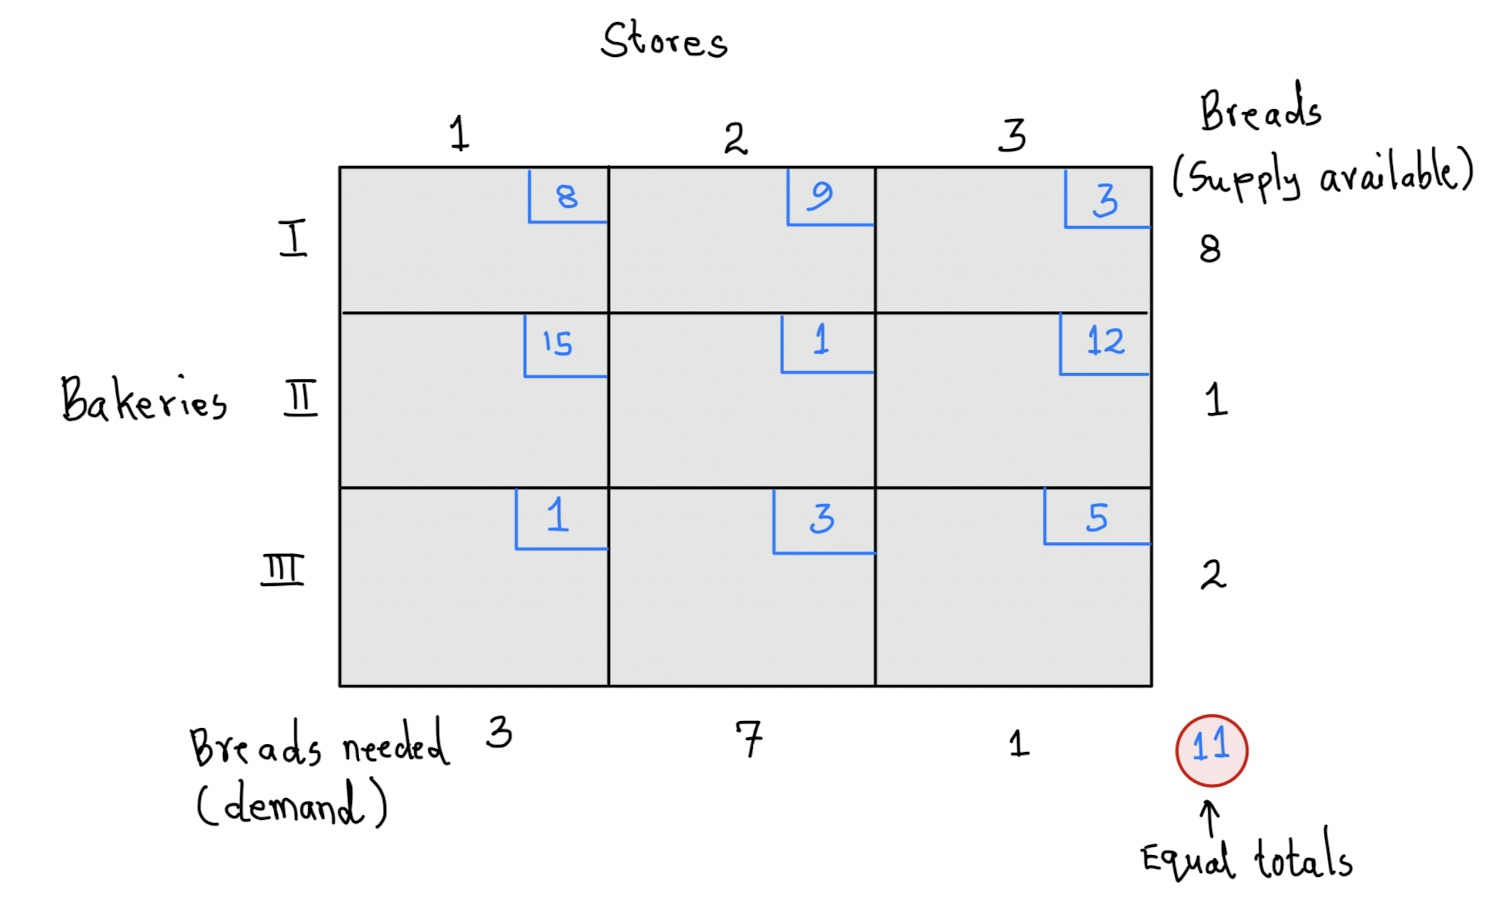
\includegraphics{images/j.jpeg} The supply available is shown on the
  right side (8,1, and 2) while the demand is shown on the bottom side
  (3, 7, and 1) of the tableau. The supply adds up to 11 and so does the
  demand. Thus, the rim conditions are satisfied. Each square on the
  tableau is called a cell and it shows the transportation cost. For
  example, the transportation cost from bakery I to store 2 is 9 units.
  We reference this cell as \((I,2)\). Similarly, in cell \((III,2)\) we
  see that the cost of transporting a dozen of bread from bakery III to
  store 2 is 5 units.
\item
  Before you learn about an algorithm that guarantees an optimal
  solution, let us look at one possible solution (feasible solution).
  Take a look at the tableau below:
\end{enumerate}

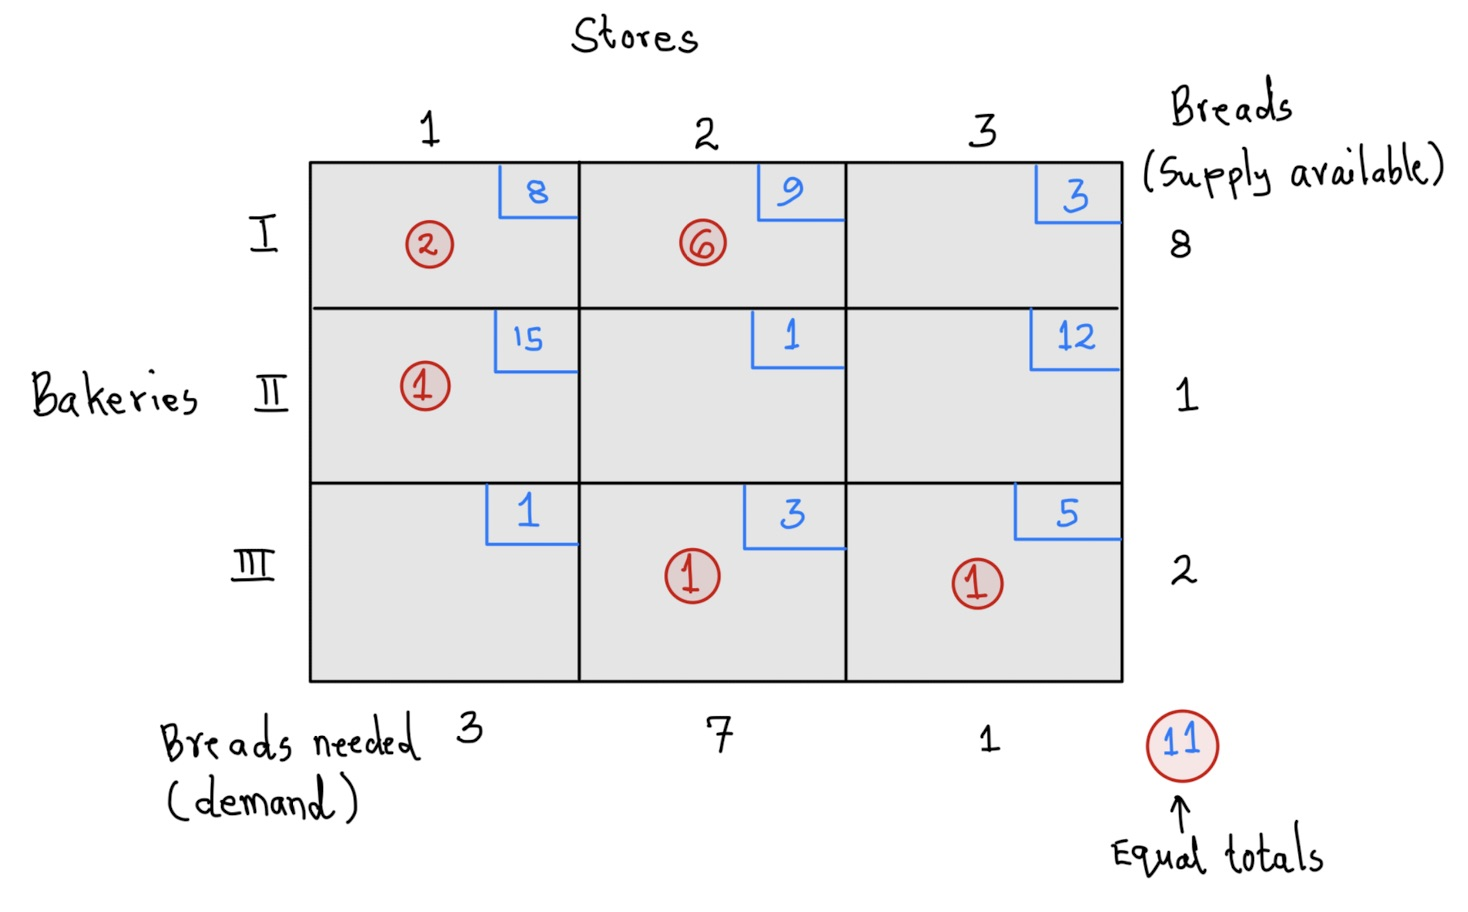
\includegraphics{images/k.jpeg} Here are important things to note about
this new tablea:

\begin{itemize}
\item
  We have new numbers (circled) added in different cells of the tableau.
  These numbers show the amount that we plan to ship. For example, the
  circled 6 in cell \((I,2)\) means we plan to ship 6 units from bakery
  I to store 2.
\item
  When you add the circled numbers across rows, you get the number of
  supply for that bakery For example, the sum of the numbers in row 1
  (bakery I) is \(2+6=8\) which equals the supply that can come from
  store I.
\item
  When you add the circled numbers along columns, you get the number
  demanded by that store. For example, the sum of the circled numbers in
  column 3 is \(6+1=7\) which equals the demand for store 2.
\item
  There are only 5 circled numbers and the table has 3 columns and 3
  rows for a total of - This will always be true for any feasible
  solution.

\begin{Shaded}
\begin{Highlighting}[]
\DataTypeTok{Any} \DataTypeTok{feasible} \DataTypeTok{solution} \DataTypeTok{for} \DataTypeTok{a} \DataTypeTok{tableau} \DataTypeTok{with} \DataTypeTok{m} \DataTypeTok{rows} \DataTypeTok{and} \DataTypeTok{n} \DataTypeTok{columns} \DataTypeTok{will} \DataTypeTok{ship} 
\DataTypeTok{through} \ErrorTok{(}\DataTypeTok{m}\ErrorTok{+}\DataTypeTok{n}\ErrorTok{)}\DataTypeTok{{-}1} \DataTypeTok{cells}\KeywordTok{.} 
\end{Highlighting}
\end{Shaded}
\end{itemize}

Thus, the above shipment plan is feasible. The cost associated with the
plan is \begin{align}
Shipment \hspace{.05in}Cost&= 2(8)+6(9)+1(15)+1(3)+1(5)\\
&=16+54+15+3+5\\
&=93
\end{align}

In case you are wondering how we came up with the above shipment plan,
it means you are paying close attention. That is a good thing. The next
section presents a method know as \textbf{Northwest corner rule} that we
can use to find a feasible solution. the method does not use the
associated costs and so may not guarantee an optimal solution.

\hypertarget{the-northwest-corner-rule}{%
\section{The Northwest Corner Rule}\label{the-northwest-corner-rule}}

The northwest corner rule (NWCR) leverages the geometry of the table to
identify a feasible shipment plan. It works by reducing the initial
tableau step by step until one cell remains. Below are the steps of the
rule:

\begin{itemize}
\tightlist
\item
  On the initial tableau, locate the cell that is as far to the top and
  to the left as possible (northwest). Ship via this cell the smaller of
  the two rim values (call this \(s\)) associated with the row and
  column of the cell. Put a circled entry (the \(s\)) in this cell to
  indicate that it is in use.
\item
  Cross out the column or row that had the value \(s\) and reduce the
  other rim value by \(s\).
\item
  When a single cell remains, there will be a tie for the rim conditions
  of both the row and the column involved, and this amount is entered
  into the cell and circled.
\end{itemize}

\textbf{Example 2}

Use the \textbf{northwest corner rule} to find a feasible solution for
the tableau in example 1 above.

\textbf{\emph{Solution}}

First, recall that the NWCR ignores the costs. So, we first rewrite the
tableau without the costs. We have also removed the tableau labels for
simplicity, 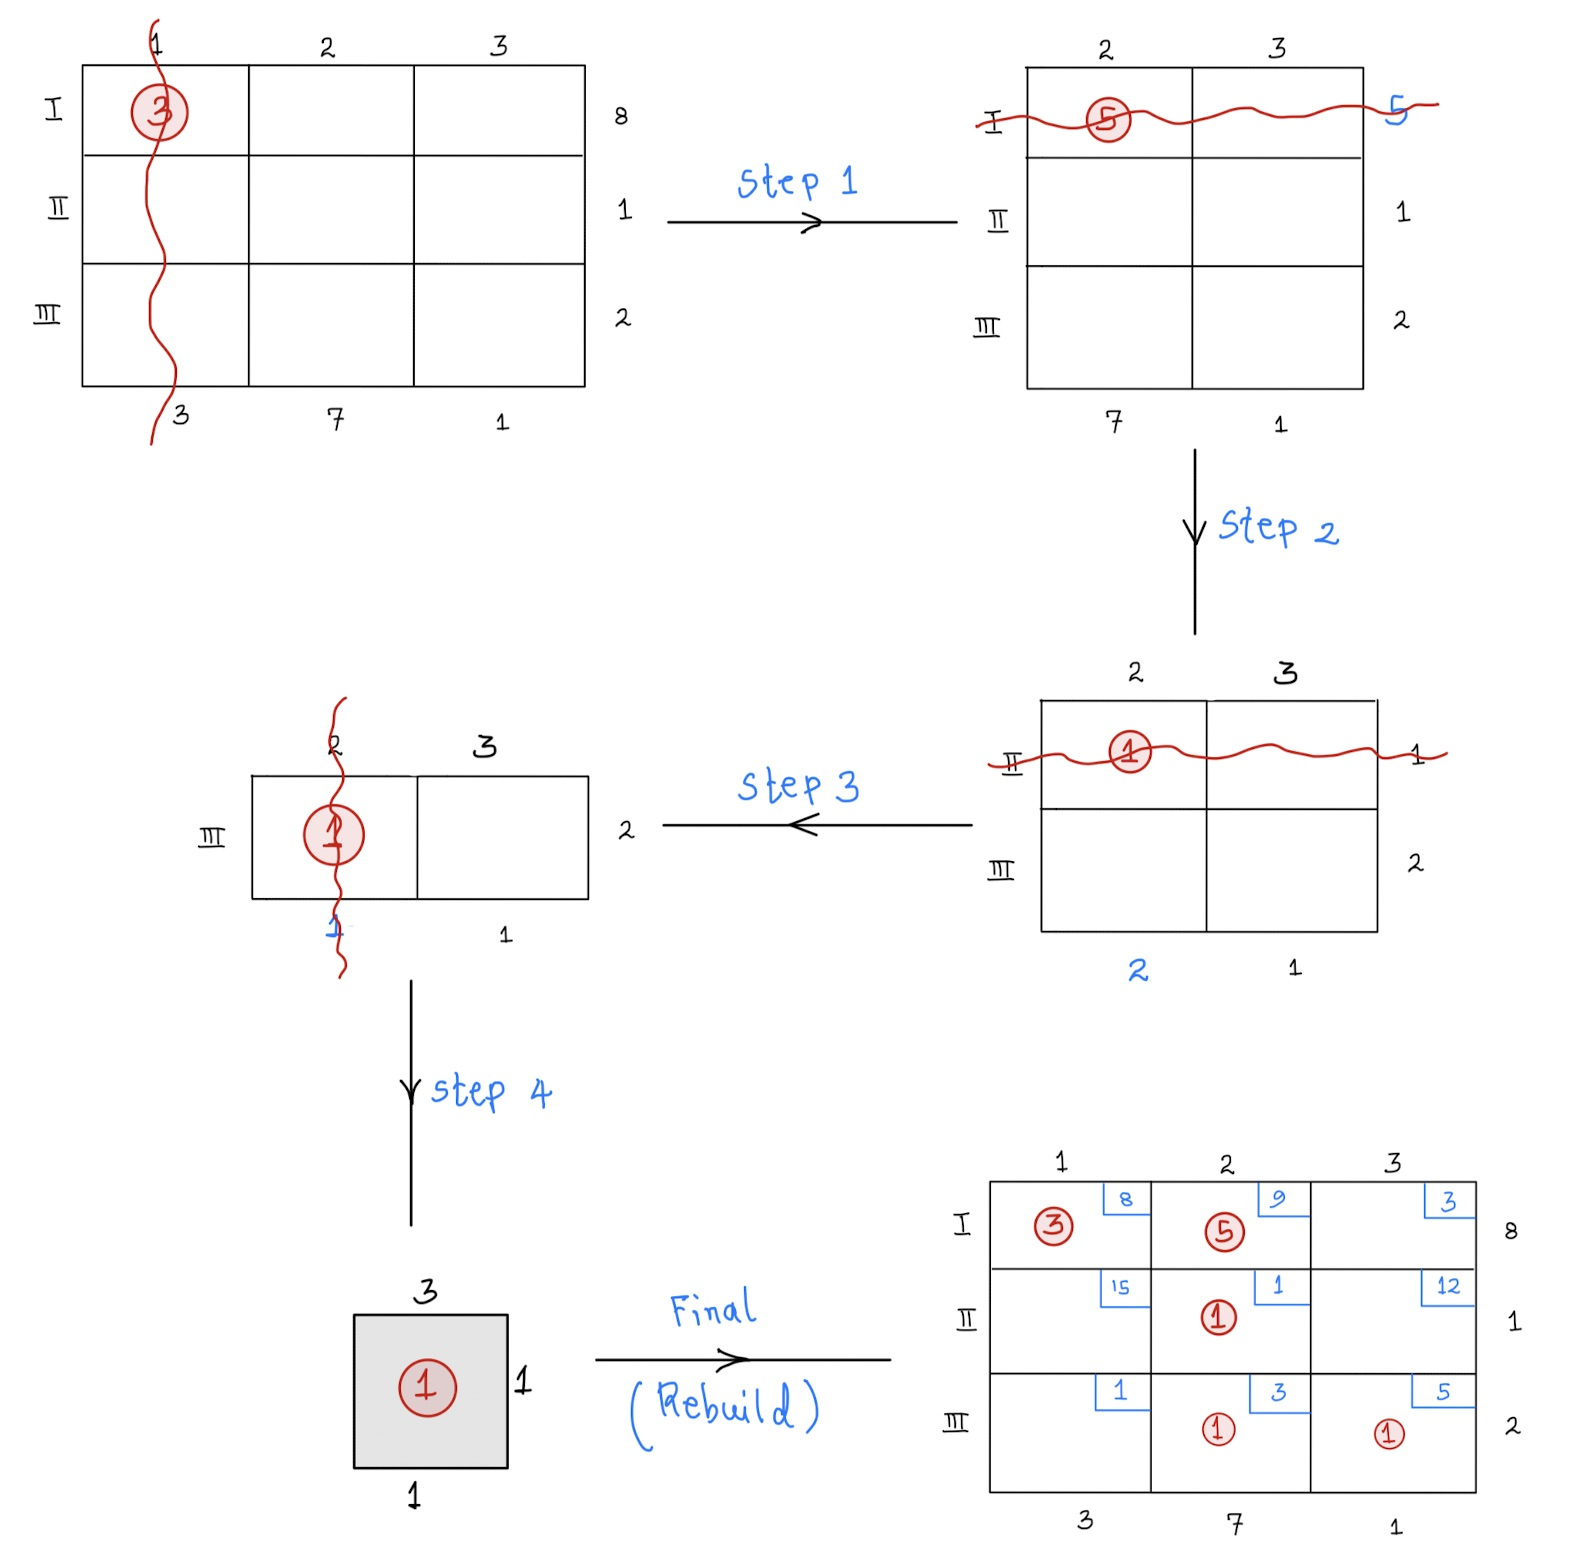
\includegraphics{images/l.jpeg}

Here is an explanation of every step:

\begin{itemize}
\item
  \textbf{\emph{Step 1:}} Locate the northwest corner cell on the
  initial tableau and ship 3 units through it. We choose 3 because it is
  the less of 3 and 8. We erase column 1 and reduce the 8 by 3.
\item
  \textbf{\emph{Step 2:}} For our new tableau (without column 1), we
  ship 5 units through the northwest cell. Delete the row and subtract 5
  from 7 to get 2.
\item
  \textbf{\emph{Step 3:}} Ship one unit through the cell shown and
  subtract the 1 from 2. Delete the row.
\item
  \textbf{\emph{step 4:}} Ship 1 unit through the northwest cell and
  erase the column. Reduce the row value by 1 to get 1. Now you are left
  with only one cell through which you ship 1 unit. You are done!
\item
  \textbf{\emph{step 5:}} Rebuild the tables with the shipments above.
\end{itemize}

Observe that there are exactly 5 cells through which we are shipping.
This is one less than 6, which is the total number of rows and columns.

The cost of this new shipment plan is,

\[
\begin{aligned}
Shipment \hspace{.05in}Cost&= 3(8)+5(9)+1(1)+1(3)+1(5)\\
&=24+45+1+3+5\\
&=78
\end{aligned}
\] Notice that this cost is smaller than what we had earlier (93). The
question that still remains is,

\textbf{\emph{Is this the cheapest solution? How can we be absolutely
sure about this?}}

It turns out that this is still \textbf{\emph{not the cheapest}}. There
is an algorithm called the \textbf{\emph{Stepping Stone Method}} that
will guarantee an optimal solution (i.e., the cheapest shipment plan).

\hypertarget{the-stepping-stone-method}{%
\section{The Stepping Stone Method}\label{the-stepping-stone-method}}

Before we look at the stepping stone method, we define the term
\textbf{\emph{indicator value}}.

\textbf{\emph{Definition:}}

The indicator values of a cell, \(C\) not currently circled is the cost
change associated with increasing or decreasing the amounts shipped in a
circuit of cells starting at cell \(C\). It is computed by summing with
alternating signs the cost of the cells in the circuit.

\textbf{\emph{Example 3}}

Since our ultimate goal is to improve the solution in the previous
example, we are going to use the final tableau earlier (left side of
figure below) to compute the indicator value. Suppose we want the
indicator value for cell \((I, 3)\). Notice that this cell is currently
not circled.

\begin{figure}

{\centering 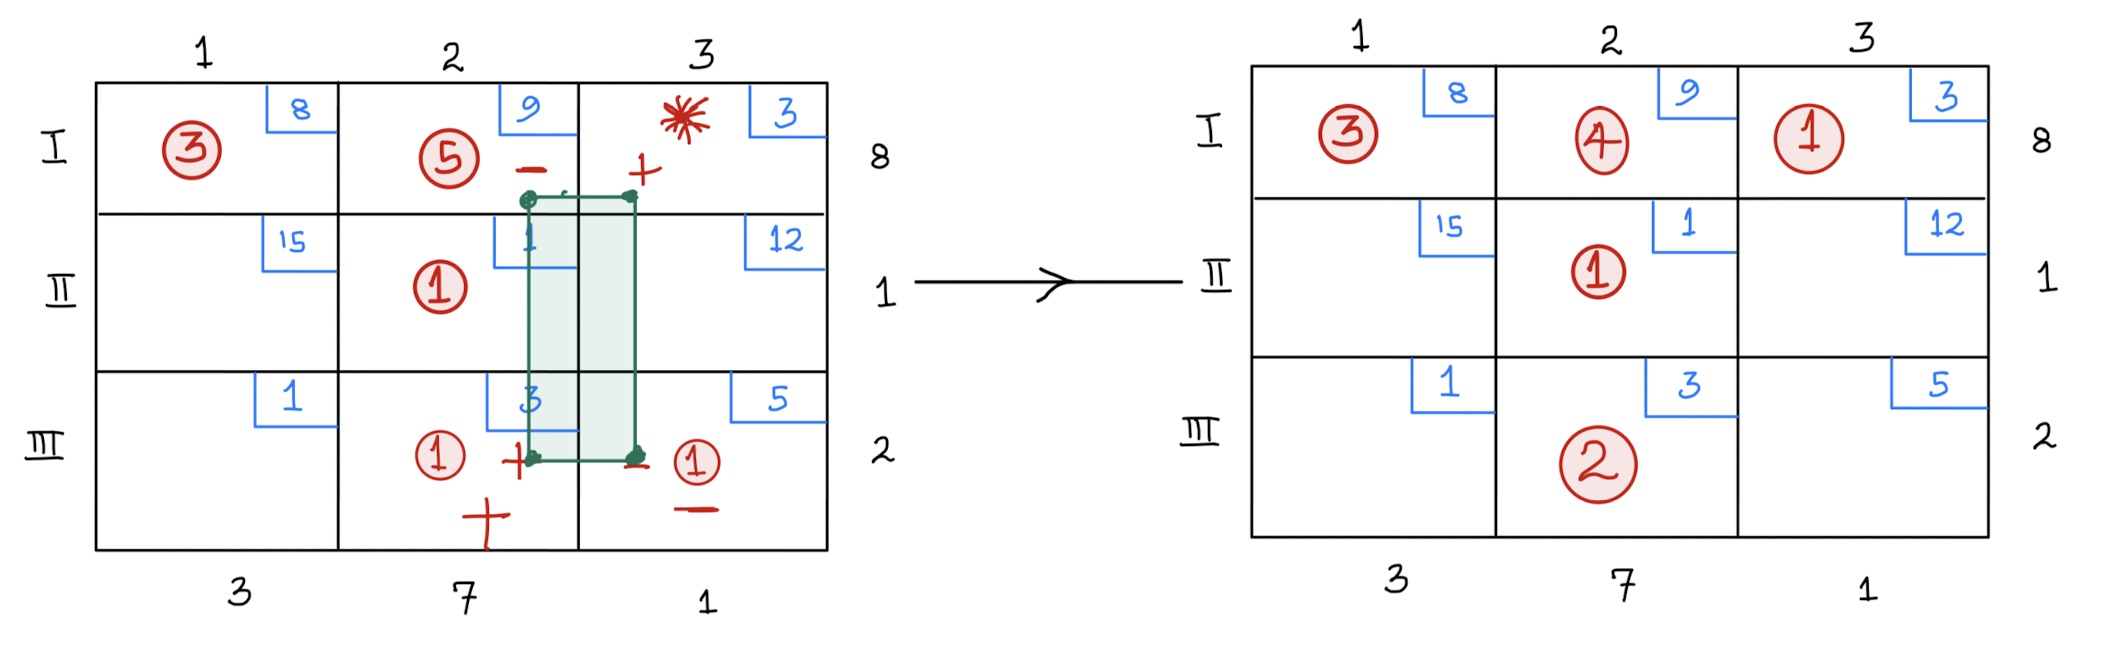
\includegraphics{images/m.jpeg}

}

\caption{First tableau}

\end{figure}

Notice that the circuit has alternating \(+\) and \(-\) signs. We can
ship \(1\) unit through cell \((I,3)\) and then reduce the amount being
shipped in cell \((III,3)\) by \(1\). This means we reduce the amount in
cell \((I,2)\) by \(1\) and then increase the amount being shipped in
cell \((III,2)\) by \(1\) unit. Doing this does not affect the
\textbf{\emph{rim conditions}} (look at the new tableau).

By using this alternative tableau, we get a cost of \(70\). See below:

\[
\begin{aligned}
Shipment \hspace{.05in}Cost&= 3(8)+4(9)+1(1)+2(3)+1(3)\\
&=24+36+1+6+3\\
&=70
\end{aligned}
\] The difference in cost between this new tableau and the original one
is \(-8\). Thus, the indicator value of this cell is \(-8\).

Alternatively, we can compute the indicator values directly from the
circuit as follows:

\[
\begin{aligned}
Indicator \hspace{.05in}Value&= 1(3)-1(9)+1(3)-1(5)\\
&=3-9+3-5\\
&=-8
\end{aligned}
\] We use 1 unit for each cell cost because that is the amount we are
moving around thr circuit.

Some things to Note;

\begin{itemize}
\tightlist
\item
  Example 3 above shows that by moving things around via the indicator
  value, we can save on the transportation cost.
\item
  The maximum amount you can move around is capped on the amount that
  can be shipped via a given cell. In our example above, we moved only 1
  because that is the maximum that can be shipped via cell \((I,3)\). If
  you move 2 for example, you will violate the rim conditions.
\item
  The indicator value of a cell tells you the amount by which the cost
  decreases or increases if you ship via that cell.
\item
  You start with an empty cell but all the other three cells in the
  circuit must have some shipment already.
\item
  In some cases, we can ship 0 quantities through a cell.
\end{itemize}

Now, we need to compute the indicator values for the rest of the cells.

Indicator value computation for cell \((II,3)\) is shown below:
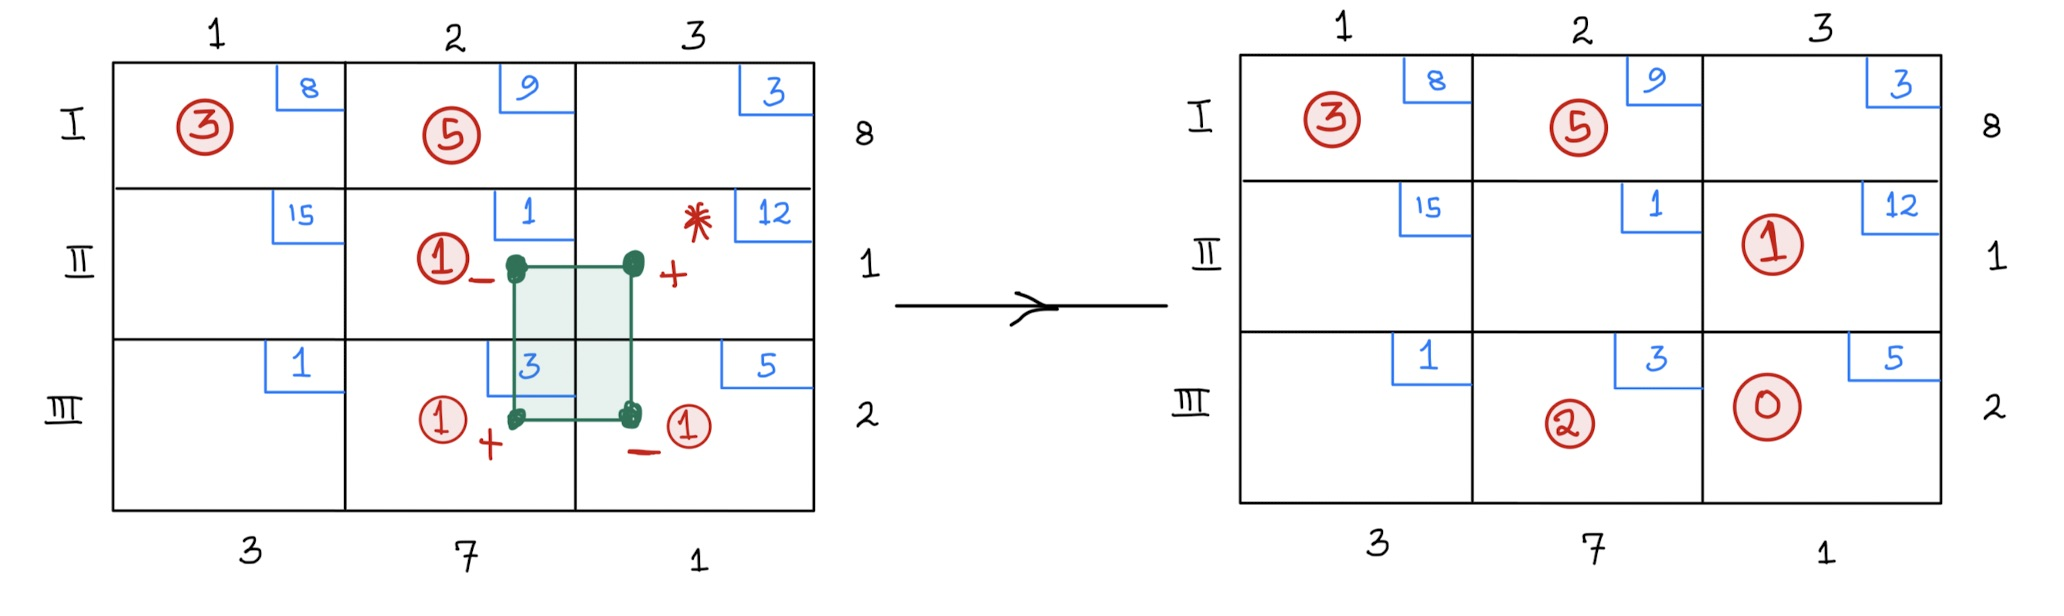
\includegraphics{images/n.jpeg}

\[
\begin{aligned}
Indicator \hspace{.05in}Value&= 1(12)-1(1)+1(3)-1(5)\\
&=12-1+3-5\\
&=+9
\end{aligned}
\] The positive indicator value means that shipping through that cell
adds the cost. So, this does not help.

Notice that the indicator values for the other two cells based on our
initial tableau are also positive. So, our best tableau at the moment is
the second figure in example 3 above. We ask ourselves, can we improve
this tableau any further? It turns out that the only cell with negative
indicator value based this new tableau is \((III, 1)\). See figure
below:

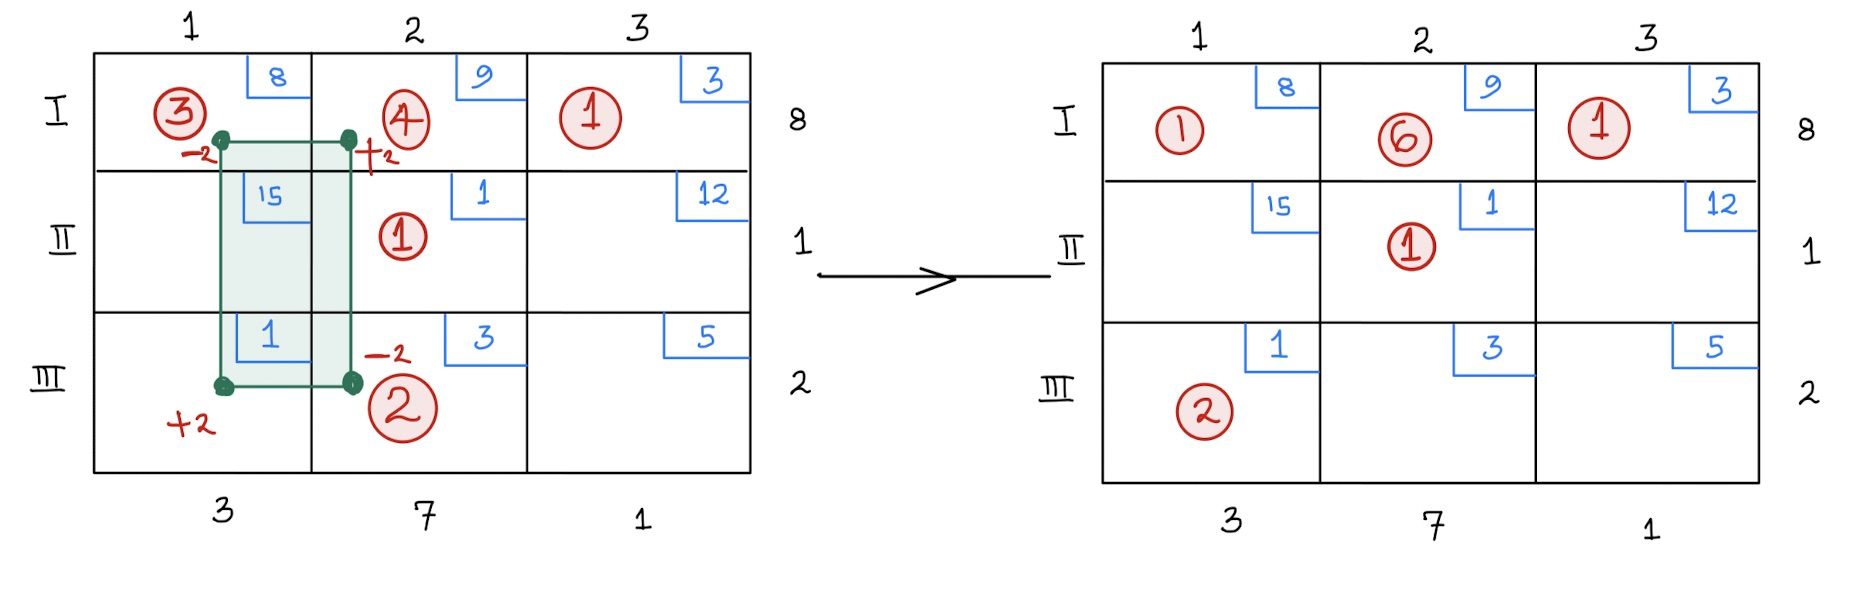
\includegraphics{images/o.jpeg} Notice that we moved 2 units around this
time.

With this new tableau, all the empty cells have positive indicator
values and so we cannot improve any further. We now have an
\textbf{\emph{optimal shipping plan}}. The cost of the plan is

\[
\begin{aligned}
Shipment \hspace{.05in}Cost&= 1(8)+6(9)+1(3)+1(1)+2(1)\\
&=8+54+3+1+2\\
&=68
\end{aligned}
\] The above process is called the \textbf{\emph{stepping stone
method}}. You check indicator values at every step until all cells have
positive indicators values, which means the solution cannot be improved
any further.

\textbf{Example 4} (Adopted from \emph{For All Practical Purposes, 10th
Edition})

Two dairies supply three supermarket chains with the demands for sour
cream as shown in the tableau below. Also indicated in the cells is the
cost of shipping between pairs of sites.

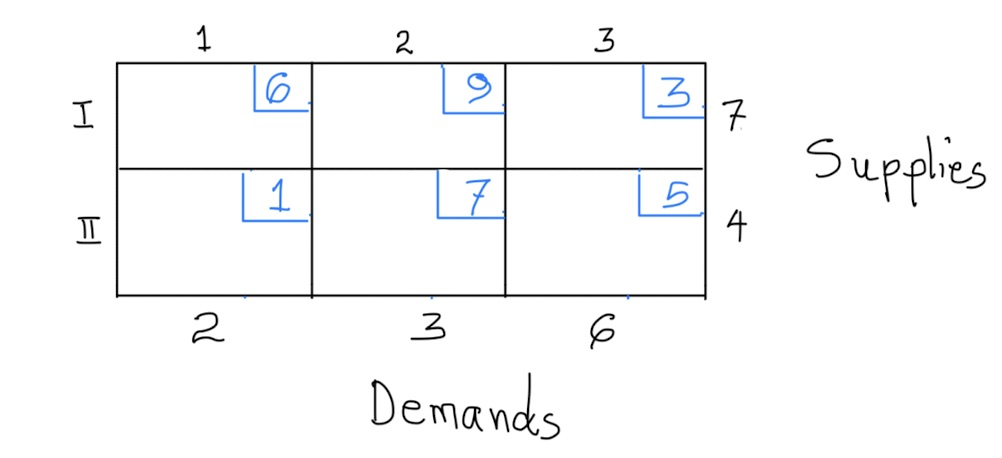
\includegraphics[width=0.7\textwidth,height=\textheight]{images/p.jpeg}

a) Use the Northwest Corner Rule to obtain a feasible solution, and
compute the cost of this feasible solution.

b) If the feasible solution in part (a) is not optimal, find an optimal
solution.

\textbf{\emph{Solution}}

Applying the northwest corner rule, we get the following tableau:
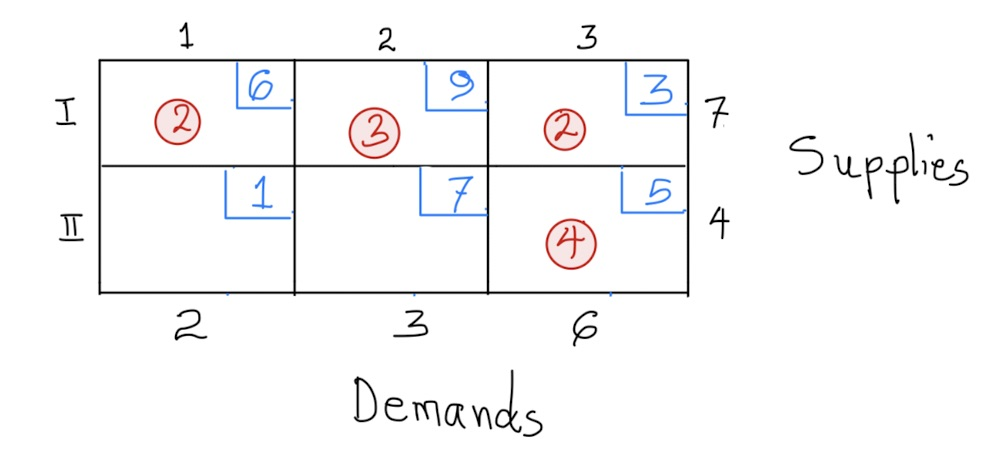
\includegraphics[width=0.7\textwidth,height=\textheight]{images/q.jpeg}

a) Note that the rim conditions are satisfied. The solution for this
shipping plan would be \[
\begin{aligned}
Cost&=2(6)+3(9)+2(3)+4(5)\\
&= 12+27+6+20\\
&=65
\end{aligned}
\] b) To determine whether the solution in (a) is optimal, we compute
the indicator values for each of the empty cells:

For cell \((II,1)\),

\[
\begin{aligned}
Indicator \hspace{.05in}Value
&=+1-6+3-5\\
&=-7
\end{aligned}
\]

For cell \((II,2)\),

\[
\begin{aligned}
Indicator \hspace{.05in}Value
&=+7-5+3-9\\
&=-4
\end{aligned}
\] The negative indicator values mean that the solution we have is not
optimal. We can improve it.

Let us ship via \((II,1)\). The new tableau for this plan is,
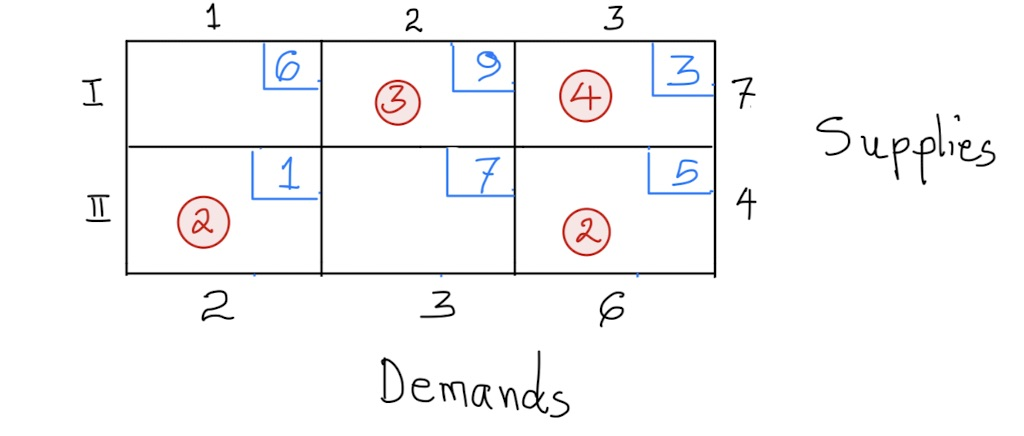
\includegraphics[width=0.7\textwidth,height=\textheight]{images/s.jpeg}

And the associated cost is,

\[
\begin{aligned}
Shipment \hspace{.05in}Cost
&=2(1)+2(5)+5(3)+3(9)\\
&=51
\end{aligned}
\] Although this is an improved solution, the indicator value for cell
\((II,2)\) is negative \((7-5+3-9=-4)\), which means we can do better.

Let us improve this by shipping via cell \((II,2)\). The new tableau
becomes,
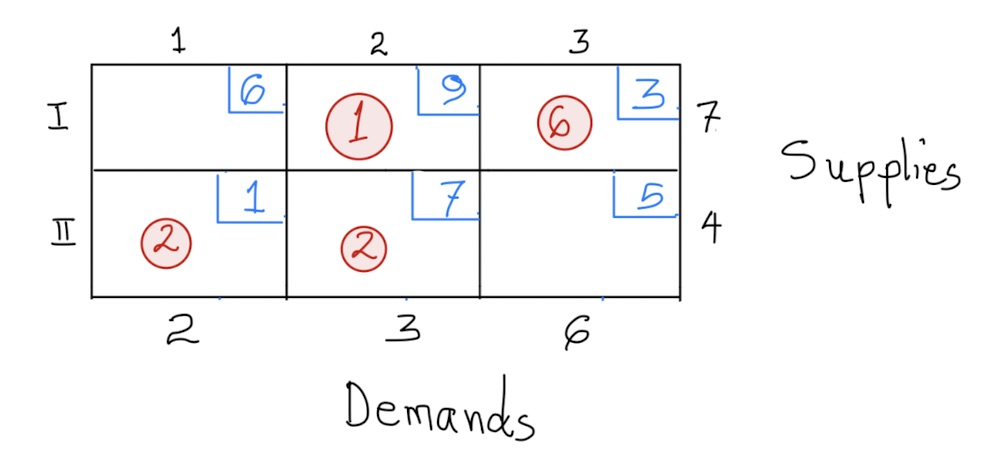
\includegraphics[width=0.7\textwidth,height=\textheight]{images/r.jpeg}

Notice that with this new tableau, all empty cells have positive
indicator values. Hence, this is the best shipment plan that we can get
and thus is the optimal solution.

The cost associated with this plan is,

\[
\begin{aligned}
Shipment \hspace{.05in}Cost
&=2(1)+2(7)+6(3)+1(9)\\
&=43
\end{aligned}
\]

\hypertarget{exercises-4}{%
\section{Exercises}\label{exercises-4}}

\begin{enumerate}
\def\labelenumi{\arabic{enumi}.}
\tightlist
\item
  For each of the following tableaux, create a possible real-world
  setting for the problem.
\end{enumerate}

\begin{enumerate}
\def\labelenumi{\alph{enumi})}
\tightlist
\item
\end{enumerate}

\begin{figure}

{\centering 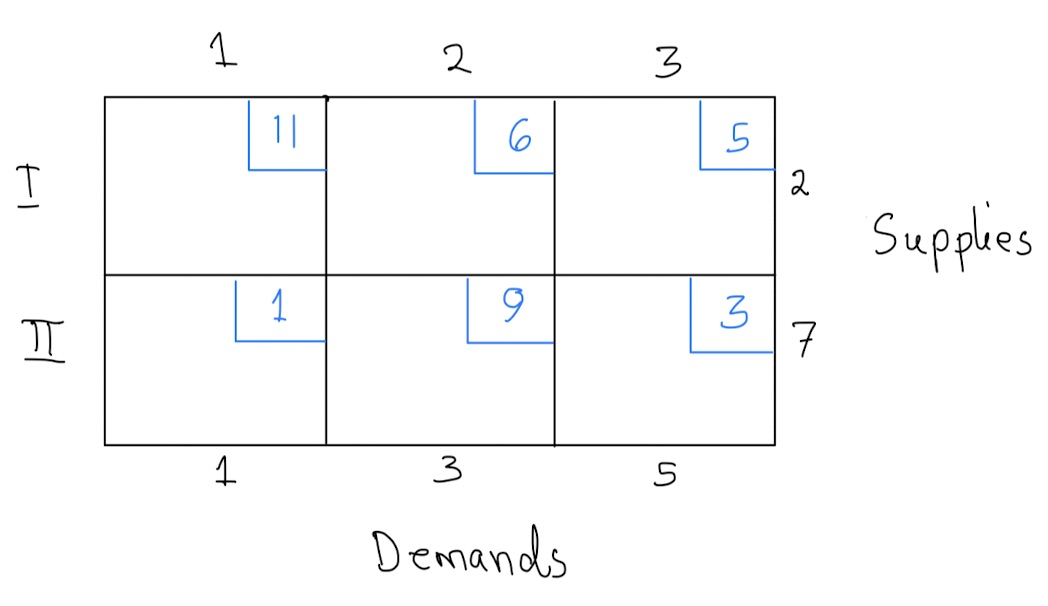
\includegraphics[width=0.6\textwidth,height=\textheight]{images/t1.jpeg}

}

\end{figure}

\begin{enumerate}
\def\labelenumi{\alph{enumi})}
\setcounter{enumi}{1}
\tightlist
\item
\end{enumerate}

\begin{figure}

{\centering 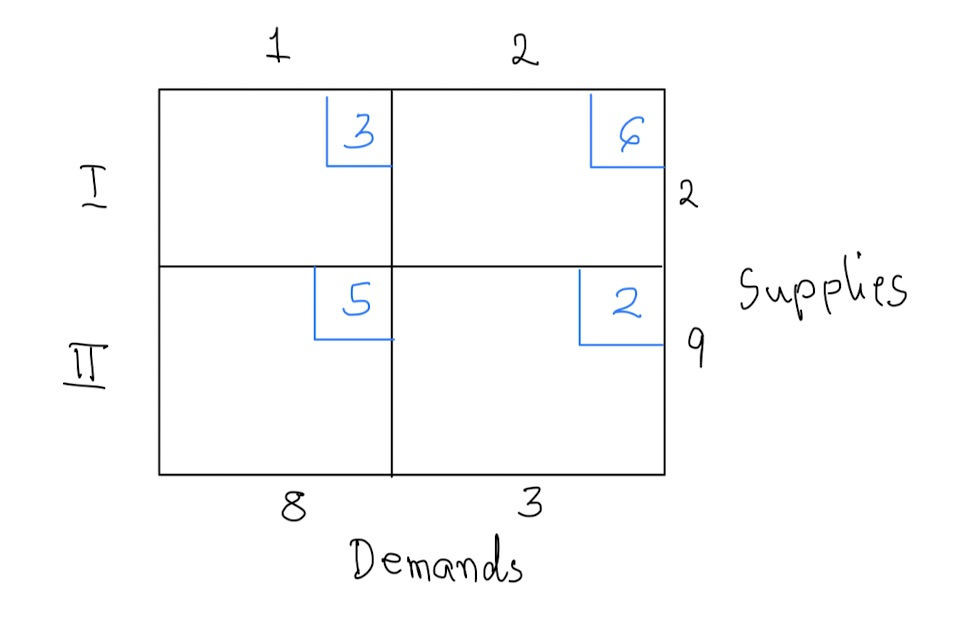
\includegraphics[width=0.6\textwidth,height=\textheight]{images/t2.jpeg}

}

\end{figure}

\begin{enumerate}
\def\labelenumi{\arabic{enumi}.}
\setcounter{enumi}{1}
\item
  Use the northwest corner rule to find a feasible solution for each
  tableau in problem 1 above. Note that the solution need not be
  optimal.
\item
  The following tableau represents the shipping costs and
  supply-and-demand constraints for supplies of oranges to juice
  manufacturing
  companies.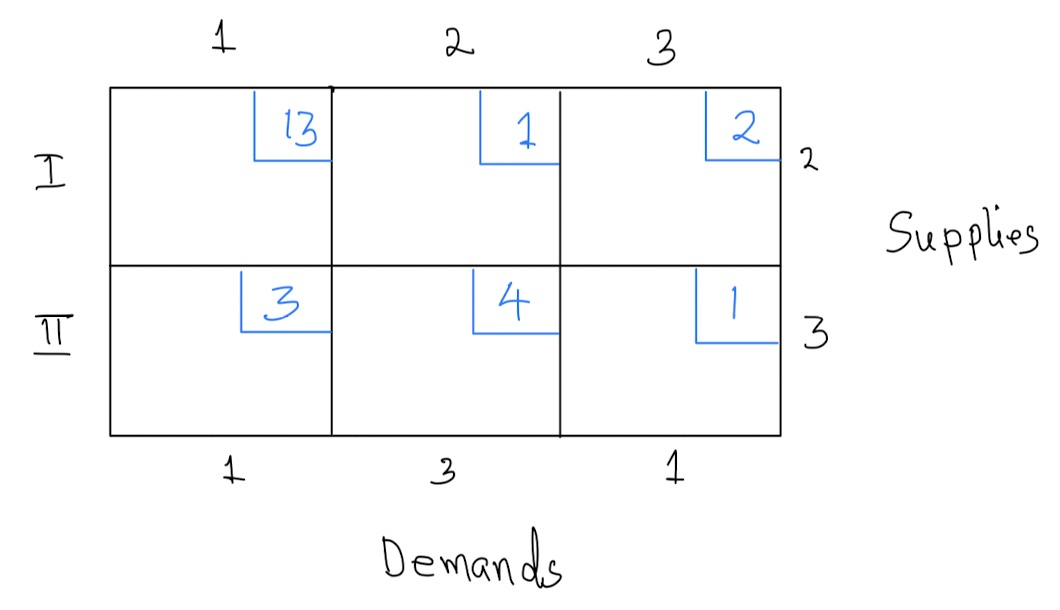
\includegraphics[width=0.6\textwidth,height=\textheight]{images/t3.jpeg}

  \begin{enumerate}
  \def\labelenumii{\alph{enumii})}
  \tightlist
  \item
    Using the northwest corner rule, find the initial solution.
  \item
    Calculate the indicator value for each non-circled cell.
  \item
    Is the current solution optimal?
  \item
    If your answer to part (c) above is ``NO'', find an optimal
    solution.
  \end{enumerate}
\item
  The following tableau shows the cost of returning cars from cities
  that have more cars than necessary to cities that have too few
  cars.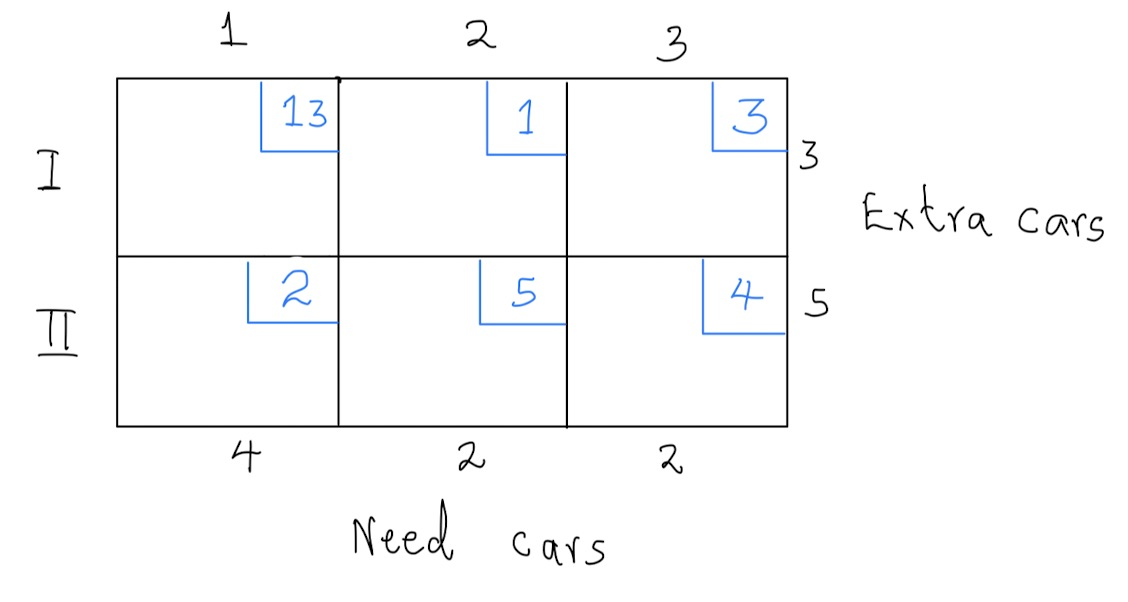
\includegraphics[width=0.6\textwidth,height=\textheight]{images/t4.jpeg}

  \begin{enumerate}
  \def\labelenumii{\alph{enumii})}
  \tightlist
  \item
    Find an initial shipment plan
  \item
    Compute the cost of the plan in (a) above.
  \item
    Determine if the solution found in (b) is optimal. If the solution
    is not optimal, find an optimal solution.
  \end{enumerate}
\item
  Consider the tableau below
  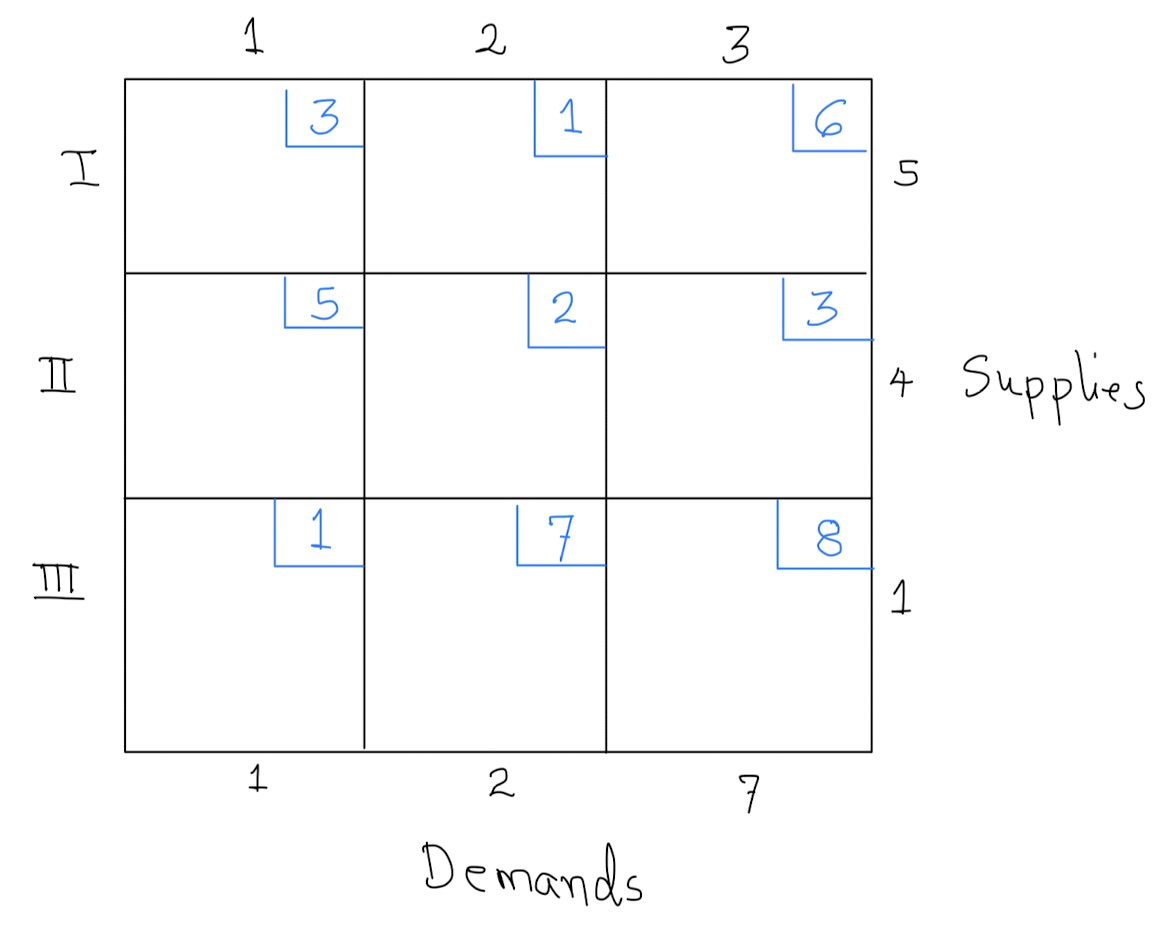
\includegraphics[width=0.6\textwidth,height=\textheight]{images/t5.jpeg}

  \begin{enumerate}
  \def\labelenumii{\alph{enumii})}
  \tightlist
  \item
    Apply the northwest corner rule to the following tableau
  \item
    Find the cost associated with the solution in (a) above.
  \item
    Compute the indicator value for each non circled cell.
  \item
    Is the solution found in part (b) optimal? If not, find an optimal
    solution.
  \end{enumerate}
\end{enumerate}

\part{Mathematics of Finance}

\hypertarget{simple-interest}{%
\chapter{Simple Interest}\label{simple-interest}}

\hypertarget{compound-interest}{%
\chapter{Compound Interest}\label{compound-interest}}

\hypertarget{annuities-and-sinking-funds}{%
\chapter{Annuities and Sinking
Funds}\label{annuities-and-sinking-funds}}

Hey Tex, this is an empty document.

\bookmarksetup{startatroot}

\hypertarget{summary}{%
\chapter{Summary}\label{summary}}

In summary, this book has no content whatsoever.

\begin{Shaded}
\begin{Highlighting}[]
\DecValTok{1} \SpecialCharTok{+} \DecValTok{1}
\end{Highlighting}
\end{Shaded}

\begin{verbatim}
[1] 2
\end{verbatim}

\bookmarksetup{startatroot}

\hypertarget{references}{%
\chapter*{References}\label{references}}
\addcontentsline{toc}{chapter}{References}

\markboth{References}{References}

\hypertarget{refs}{}
\begin{CSLReferences}{1}{0}
\leavevmode\vadjust pre{\hypertarget{ref-knuth84}{}}%
Knuth, Donald E. 1984. {``Literate Programming.''} \emph{Comput. J.} 27
(2): 97--111. \url{https://doi.org/10.1093/comjnl/27.2.97}.

\end{CSLReferences}



\end{document}
